% Sablon pentru realizarea lucrarii de licenta, conform cu recomandarile
% din ghidul de redactare:
% - https://fmi.unibuc.ro/finalizare-studii/
% - https://drive.google.com/file/d/1xj9kZZgTkcKMJkMLRuoYRgLQ1O8CX0mv/view

% Multumiri lui Gabriel Majeri, acest sablon a fost creat pe baza
% codului sursa a lucrarii sale de licenta. 
% Codul sursa: https://github.com/GabrielMajeri/bachelors-thesis
% Website: https://www.gabrielmajeri.ro/
%
% Aceast sablon este licentiat sub Creative Commons Attribution 4.0 International License.

\documentclass[12pt, a4paper]{report}

% Suport pentru diacritice și alte simboluri
\usepackage{fontspec}

% Suport pentru mai multe limbi
\usepackage{polyglossia}

% Setează limba textului la română
\setdefaultlanguage{english}
% Am nevoie de engleză pentru rezumat
\setotherlanguages{romanian}

% Indentează și primul paragraf al fiecărei noi secțiuni
\SetLanguageKeys{english}{indentfirst=true}

% Suport pentru diferite stiluri de ghilimele
\usepackage{csquotes}

\DeclareQuoteStyle{english}
  {\quotedblbase}
  {\textquotedblright}
  {\guillemotleft}
  {\guillemotright}

% Utilizează biblatex pentru referințe bibliografice
\usepackage[
    maxbibnames=50,
    sorting=nty
]{biblatex}

\addbibresource{bibliography.bib}

% Setează spațiere inter-linie la 1.5
\usepackage{setspace}
\onehalfspacing

% Modificarea geometriei paginii
\usepackage{geometry}

% Include funcțiile de grafică
\usepackage{graphicx}
\usepackage{svg}
\usepackage{subcaption} 
\usepackage{float}
% Încarcă imaginile din directorul `images`
\graphicspath{{./images/}}

% Listări de cod
\usepackage{listings}

% Linkuri interactive în PDF
\usepackage[
    colorlinks,
    linkcolor={black},
    menucolor={black},
    citecolor={black},
    urlcolor={blue}
]{hyperref}

% Simboluri matematice codificate Unicode
\usepackage[warnings-off={mathtools-colon,mathtools-overbracket}]{unicode-math}

% Comenzi matematice
\usepackage{amsmath}
\usepackage{mathtools}

% Formule matematice
\newcommand{\bigO}[1]{\symcal{O}\left(#1\right)}
\DeclarePairedDelimiter\abs{\lvert}{\rvert}

% Suport pentru pseudocod
\usepackage{algorithm} 
\usepackage{algpseudocode} 

% Suport pentru rezumat în două limbi
% Bazat pe https://tex.stackexchange.com/a/70818
\newenvironment{abstractpage}
  {\cleardoublepage\vspace*{\fill}\thispagestyle{empty}}
  {\vfill\cleardoublepage}
\renewenvironment{abstract}[1]
  {\bigskip\selectlanguage{#1}%
   \begin{center}\bfseries\abstractname\end{center}}
  {\par\bigskip}

% Suport pentru anexe
\usepackage{appendix}

% Stiluri diferite de headere și footere
\usepackage{fancyhdr}

% Pentru tabele
\usepackage{booktabs}
\usepackage{array}
\usepackage{tabularx}
\newcolumntype{C}{>{\centering\arraybackslash}X}

% Metadate
\title{Convex Optimization Relaxation for Radial Image Reconstruction}
\author{Mincu Adrian-Lucian}

% Generează variabilele cu @
\makeatletter

\begin{document}

% Front matter
\cleardoublepage
\let\ps@plain

% Pagina de titlu
\begin{titlepage}

% Redu marginile
\newgeometry{left=2cm,right=2cm,bottom=1cm}

\begin{figure}[!htb]
    \centering
    \begin{minipage}{0.2\textwidth}
        
\includegraphics[width=\linewidth]{logo-ub.png}
    \end{minipage}
    \begin{minipage}{0.5\textwidth}
        \large
        \vspace{0.2cm}
        \begin{center}
            \textbf{UNIVERSITY OF BUCHAREST}
        \end{center}
        \vspace{0.3cm}
        \begin{center}
            \textbf{
                FACULTY OF \\
                MATHEMATICS AND COMPUTER SCIENCE
            }
        \end{center}
    \end{minipage}
    \begin{minipage}{0.2\textwidth}
        
\includegraphics[width=\linewidth]{logo-fmi.png}
    \end{minipage}
\end{figure}

\begin{center}
\textbf{SPECIALIZATION COMPUTER SCIENCE}
\end{center}

\vspace{1cm}

\begin{center}
\Large \textbf{Bachelor's thesis}
\end{center}

\begin{center}
\huge \textbf{\MakeUppercase{\@title}}
\end{center}

\vspace{3cm}

\begin{center}
\large \textbf{Graduate \\ \@author}
\end{center}

\vspace{0.25cm}

\begin{center}
\large \textbf{Scientific coordinator \\ Conf. Dr. Rusu Cristian}
\end{center}

\vspace{2cm}

\begin{center}
\Large \textbf{Bucharest, June 2025}
\end{center}
\end{titlepage}
\restoregeometry
\newgeometry{
    margin=2.5cm
}

\fancypagestyle{main}{
  \fancyhf{}
  \renewcommand\headrulewidth{0pt}
  \fancyhead[C]{}
  \fancyfoot[C]{\thepage}
}

\addtocounter{page}{1}

% Rezumatul
\begin{abstractpage}

\begin{abstract}{english}

Radial image reconstruction is an ongoing challenge in the computational imaging field, with applications in medical tomography as well as artistic renderings. This bachelor’s thesis addresses the aforementioned problem by exploring optimization algorithms to reconstruct images from a set of radial projections. The main objective is to implement and analyze optimization algorithms, with particular attention to aspects such as time and memory consumption, as well as the visual quality of the results.

To illustrate and demonstrate our approach, we solve the string art problem\footnote{For more on string art, see \href{https://en.wikipedia.org/wiki/String_art}{String Art}}, which is a smaller subproblem of the general radial reconstruction problem. We will introduce a method commonly used in radial image reconstruction, applied in the novel context of string art, using a custom implementation of the Radon transform. Although string art is used as a conceptual analogy, the focus of this thesis lies in the mathematical and algorithmic methods for the broader problem of radial image reconstruction.

Thus, this thesis will contribute to the field of image processing while also offering a new perspective on the artistic applications of mathematics and programming.

\end{abstract}

\begin{abstract}{romanian}

Reconstrucția imaginii radiale este o problemă curentă în domeniul imagisticii computaționale, cu aplicații în tomografia medicală și în redări artistice. Această lucrare de licență abordează problema menționată anterior, explorând algoritmi de optimizare pentru reconstrucția imaginilor dintr-un set de proiecții radiale. Obiectivul principal este implementarea și analiza algoritmilor de optimizare, cu accent pe aspecte precum timpul și memoria de calcul, precum și calitatea rezultatului obținut.

Pentru a ilustra și demonstra abordarea noastră, vom rezolva problema string art\footnote{Pentru mai multe despre string art, vedeți \href{https://en.wikipedia.org/wiki/String_art}{String Art}}, care este o subproblemă a problemei generale de reconstrucție radială. Vom introduce o metodă utilizată frecvent în reconstrucția imaginii radiale, aplicată într-un context nou, cel al string art, folosind o implementare personalizată a transformatei Radon. Deși string art este folosită ca o analogie conceptuală, accentul acestei lucrări cade pe metodele matematice și algoritmice ale problemei generale de reconstrucție a imaginii radiale.

Astfel, lucrarea contribuie la domeniul procesării imaginilor, oferind și o perspectivă nouă asupra aplicațiilor artistice ale matematicii și programării.

\end{abstract}

\end{abstractpage}

\cleardoublepage
\pagestyle{empty}
\tableofcontents
\cleardoublepage
\pagestyle{main}

% Main matter
\cleardoublepage
\pagestyle{main}
\let\ps@plain\ps@main

\chapter{Introduction}

\subsubsection{Motivation}
 
Radial image reconstruction is widely used today in computational imaging, such as in Computerized Tomography (CT) scans, which are essential for diagnosing diseases or injuries. The use of such CT scans has increased drastically, making this a domain worthy of exploring optimization techniques.

The mathematics community continues to engage with these problems, exploring the Fourier transform and the Radon transform, the latter of which we also use in this thesis.

Moreover, artists must intuitively find an arrangement of the string that can recreate a given image. This process can be very tedious and time-consuming, which is why we will tackle the problem of finding a mathematical method for computing string art, thus automating the process.

\subsubsection{Personal Contribution}

In the course of this thesis we read existing literature on string art \cite{towards-computational-stringart} and \cite{computational-stringart} as well as computational optimization techniques \cite{convex-optimization}. In addition, we implemented several optimization algorithms and adapted the well known Radon transform specifically for the string art context. We designed and executed experiments to evaluate the performance of these methods and the visual quality of the results, analyzing each algorithm's strengths and limitations. Additionally, we implemented a Python package\footnote{The package is publicly available at \href{https://github.com/skpha13/cvx-rayopt}{cvx-rayopt}} containing all the methods and experiments, ensuring the reproducibility of the results through clear documentation and organized code.

\subsubsection{Structure}

We will begin by establishing a foundation of mathematical formulas and concepts in the \textit{Preliminary} section, which will serve as the basis for the methods presented later. Next, we will explore all of the optimization algorithms implemented in the \textit{Methodology} chapter and analyze their performance and visual quality in the \textit{Performance Evaluation and Analysis} chapter. Finally, we will conclude with a summary and a discussion of potential directions for future work.

\subsubsection{Digital Interpretation of String Art}

String art is a technique for creating a visual effect by manipulating thread to reproduce an image. We will procedurally compute string art configurations from a given image, modeling this real world problem using mathematical constraints.

The objective is to replicate this effect digitally, given an input image. It is important to note that there are a multiple of methods to achieve this objective, and we will examine the more intricate details of each approach.

The definition of string art we addressed earlier will not be fully applicable when recreating the image digitally, meaning some of the original constraints will be relaxed in order to explore the possibilities and limitations of this domain. This is because our objective is to visually replicate the effect produced by the traditional method, without being limited by physical constraints, such as the use of a continuous thread.

\begin{figure}[!htb]
    \centering
    \begin{minipage}{0.48\linewidth}
        \centering
        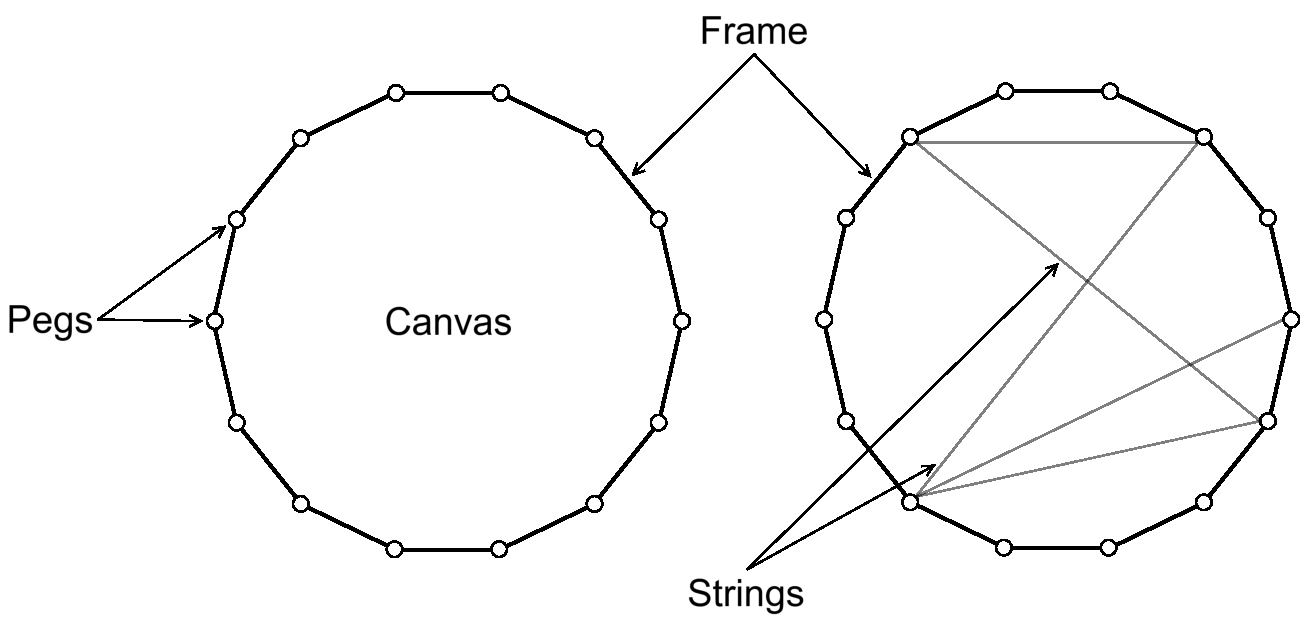
\includegraphics[width=\linewidth]{images/stringart_components.pdf}
        \caption{Image to illustrate the main components involved in creating string art patterns.}
        \label{fig:stringart_components}
    \end{minipage}
    \hfill
    \begin{minipage}{0.48\linewidth}
        \centering
        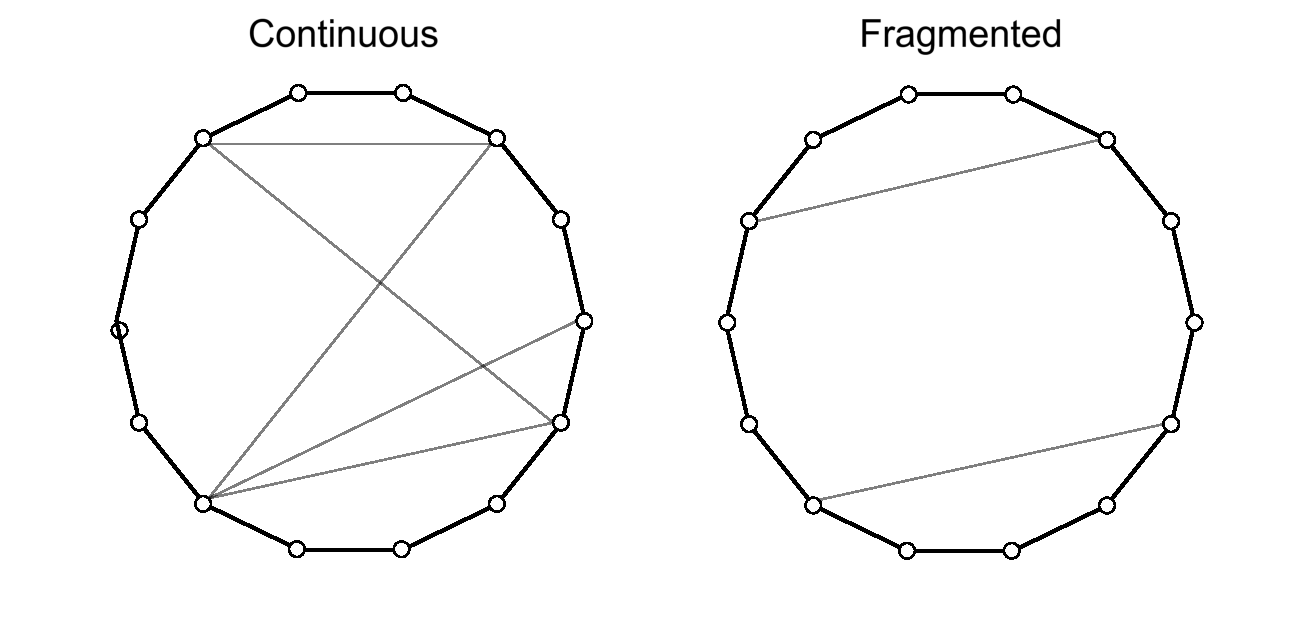
\includegraphics[width=\linewidth]{images/continuous_vs_fragmented.pdf}
        \caption{Image to illustrate the different types of arrangements: continuous versus fragmented.}
        \label{fig:continuous_vs_fragmented_strings}
    \end{minipage}
\end{figure}

Even though we are limited to drawing only straight lines, we can create the effect of a curve by drawing multiple lines that follow the trajectory of a quadratic Bézier curve. The image below illustrates this behavior.

\begin{figure}[H]
    \centering
    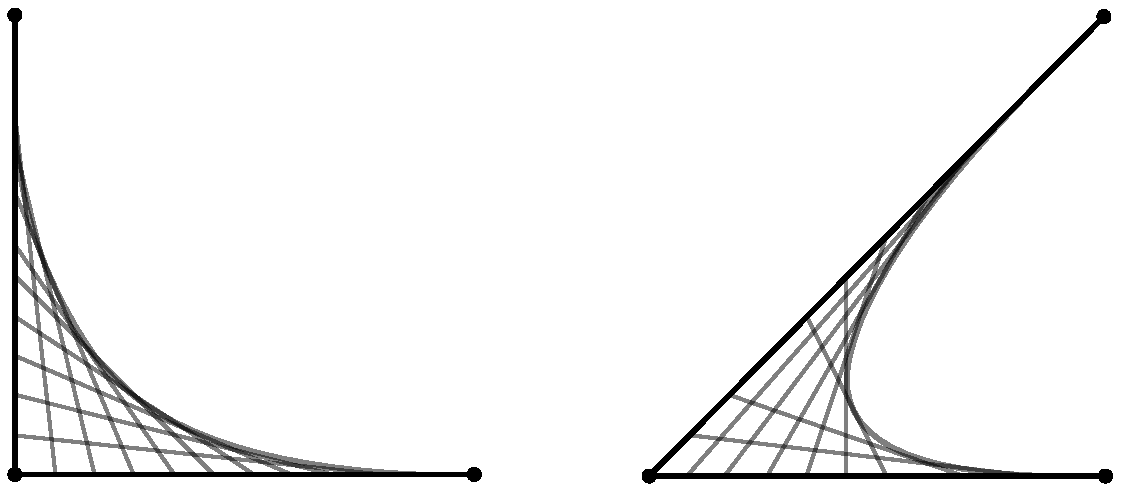
\includegraphics[width=0.5\linewidth]{images/quadratic_bezier_curves.pdf}
    \caption{Illustration of quadratic Bézier curves approximated by straight lines.}
    \label{fig:bezier_cureves}
\end{figure}
\chapter{Preliminary}

\subsubsection{Problem Formulation}
\label{sec:problem_formulation}

The input to the pipeline will be a standard image, which will first be converted to black and white, cropped into a square, and then its pixel values will be scaled to the [0,1] range. In addition, we will invert the black and white values. This is because, in traditional computer graphics, white is represented as 1 and black as 0, but our problem involves drawing thin black edges. Swapping these values promotes sparsity, which helps reduce computation time. It also aligns better with our approach, since we can \textit{add} lines together to build up the image. Lastly, we will flatten the image row-wise, and the result will be denoted as a column vector \(b \in \mathbb{R}^{m^2}\), where \(m\) is the width or height of the image.

Let \(N\) denote the number of pegs used in our computation, and let \(n = \binom{N}{2}\) the total number of possible lines that can be drawn. With this in mind, we define each matrix \(A_i\) as the matrix representing the \(i\text{-th}\) line drawn on the canvas. The final matrix \(A \in \mathbb{R}^{m^2, \space n}\) is constructed such that each column corresponds to the flattened, row-wise version of a matrix \(A_i\). This matrix \(A\) will be used in the computations that follow.

Finally, let \(x \in \mathbb{R}^n\) or \(x \in \{0, 1\}^n\) if the output vector of our solution is binary. Here, \(x_i\) indicates how much we choose to draw the \(i\text{-th}\) line, or whether we choose to draw it at all, in the binary case.

With all of the above defined, we can state our objective as minimizing the error between the string art configuration and the input image using a standard least squares formulation with the 2-norm:

\begin{equation}
\min{\| A \cdot x - b \|^2}
\label{eq:least_squares}
\end{equation}

Given the fact that the intersection of lines can create pixel values \(\geq1\) we will use a clamping function when computing the image:

\begin{equation}
y = C(Ax), \quad
C : \mathbb{R}_+^{m, \ m} \rightarrow [0, 1]^{m, \ m}, \quad
C(x) = \min(x, 1)
\label{clamping_operator}
\end{equation}

It is important to note that there exists a discrepancy in a computers perception of a \enquote{qualitative} image and the human eye. In the formula above, the computer will consider that the image with the lowest residual is the highest quality one.

\begin{figure}[H]
    \centering
    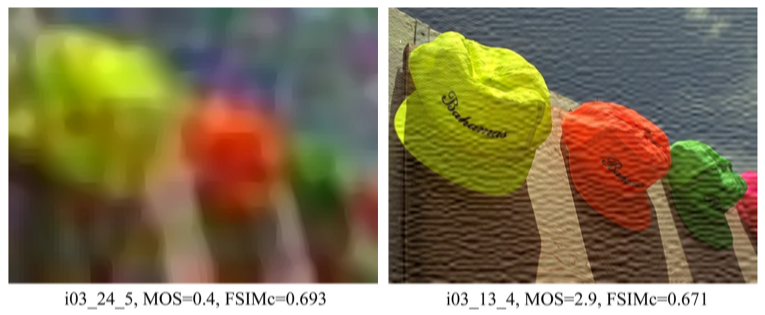
\includegraphics[width=0.66\linewidth]{perceptual_image_quality.png}
    \caption{Example from the paper \cite{perceptual_image_quality} which showcases the discrepancy between the errors given by computers and humans.}
    \label{fig:perceptual_image_quality}
\end{figure}

This phenomenon can be observed in the figure above, where the image on the left, despite having a higher FSIMc score \cite{fsimc} (the higher the better), has a lower MOS \footnote{For more details about the Mean Opinion Score (MOS), see the article on \href{https://en.wikipedia.org/wiki/Mean_opinion_score}{Mean Opinion Score (MOS)}}. This indicates that the majority of people perceived the image on the right as being of higher quality, which contradicts the result given by the computer.

\subsubsection{Peg Placement}

To place the pegs equidistantly on a circle, we used the following parametric equation of a circle.

For a circle centered at \((x_c, y_c)\) with radius \(r\) and \(N\) pegs:

\[
\begin{aligned}
x_k &= x_c + r \cdot \cos\left( \frac{2\pi k}{N} \right), \\
y_k &= y_c + r \cdot \sin\left( \frac{2\pi k}{N} \right),
\end{aligned}
\quad \text{for } k = 0, 1, 2, \dots, N - 1
\]

This placement ensures that the directions of lines connecting peg pairs are distributed uniformly over the angular domain. This is particularly important due to the Fourier Slice Theorem \footnote{For the connection between Radon and Fourier transforms, see the article on \href{https://en.wikipedia.org/wiki/Projection-slice_theorem}{Fourier Slice Theorem}}, which connects the Radon transform with the 2D Fourier transform: equidistant angular sampling allows for more accurate coverage of the frequency domain and, in turn, better image approximation through string lines.

\subsubsection{Line Rendering}

For rendering lines in the matrix representation, we initially used the Bresenham algorithm \footnote{For a detailed implementation of the algorithm, see the article on \href{https://en.wikipedia.org/wiki/Bresenham\%27s\_line\_algorithm\#Algorithm}{Bresenham's Line Algorithm}}, and later switched to the anti-aliased Xiaolin-Wu algorithm  \footnote{For a detailed implementation of the algorithm, see the article on \href{https://en.wikipedia.org/wiki/Xiaolin_Wu\%27s_line_algorithm}{Xiaolin Wu's line algorithm}}.

\chapter{Methodology}

\section{Image Preprocessing}

\begin{figure}[H]
    \centering
    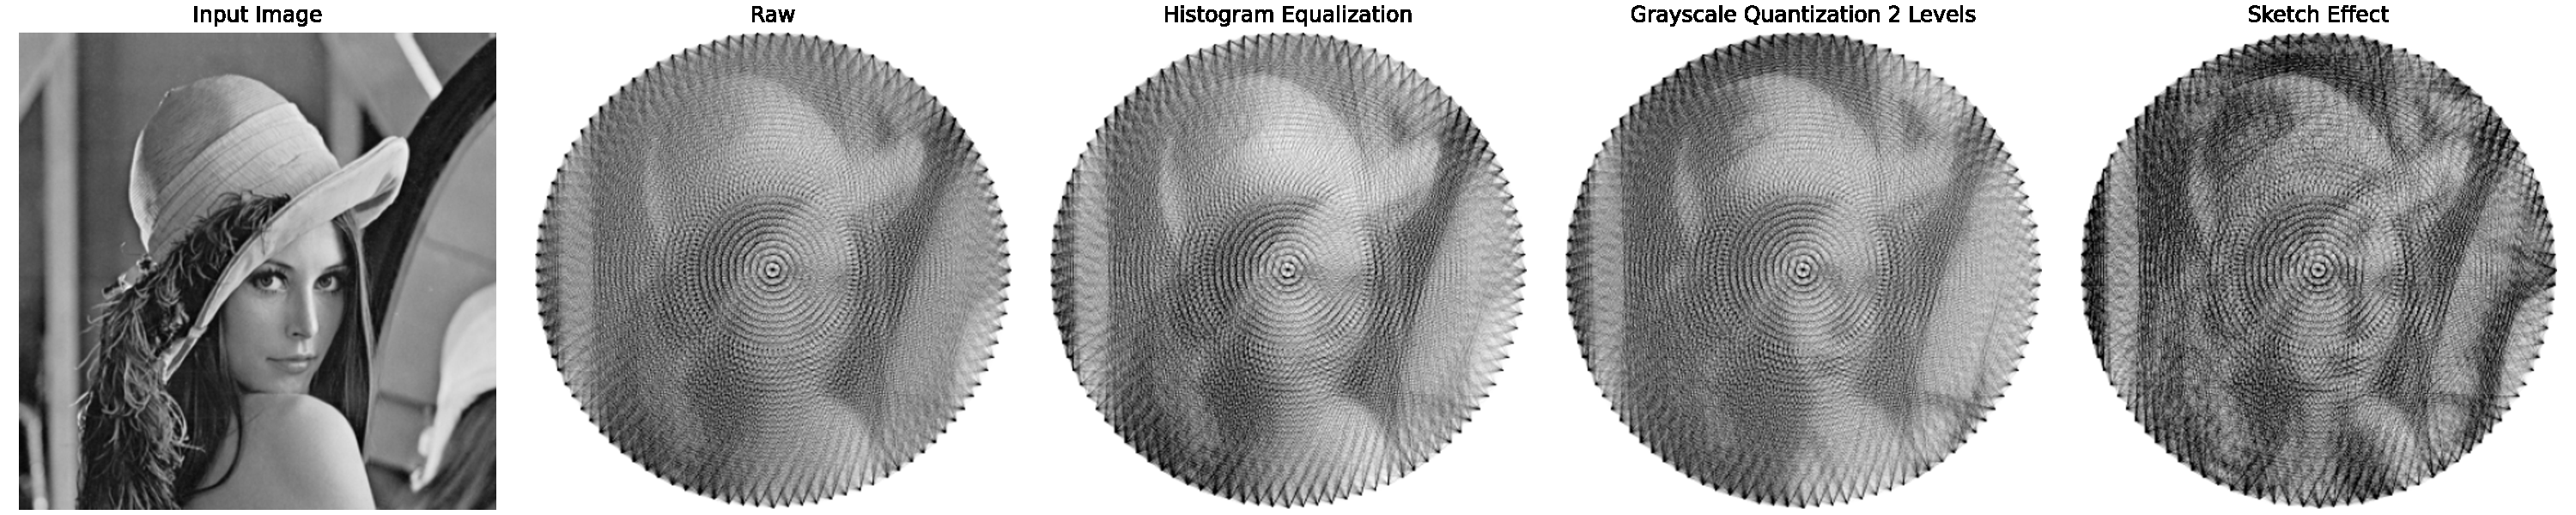
\includegraphics[width=\linewidth]{images/preprocess/preprocessed_results.pdf}
    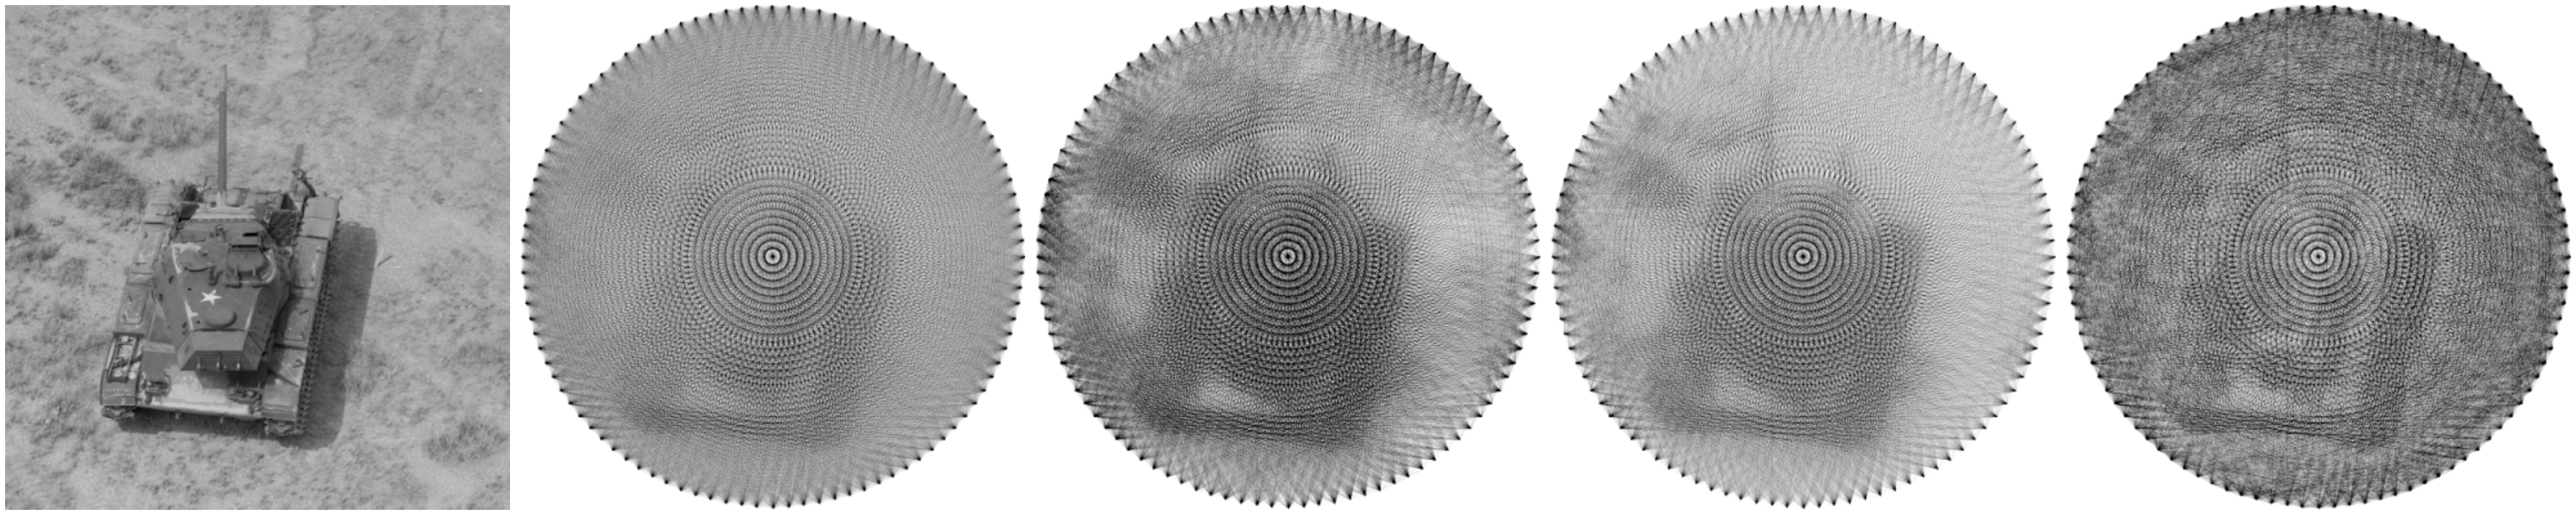
\includegraphics[width=\linewidth]{images/preprocess/preprocessed_results_tank.pdf}
    \caption{Comparative analysis of results using different preprocessing methods.}
    \label{fig:preprocess_results}
\end{figure}

Different preprocessing methods were tried, and a comparative analysis was conducted to determine the best subjective image quality. The raw result is very gray, making it somewhat difficult to distinguish details. Histogram Equalization \footnote{Details about the histogram equalization method can be found on \href{https://docs.opencv.org/4.x/d4/d1b/tutorial_histogram_equalization.html}{OpenCV: Histogram Equalization}} adds a touch of contrast, perfect in my opinion. The sketch effect \footnote{Details about the sketch effect method can be found on \href{https://medium.com/@Kavya2099/image-to-pencil-sketch-using-opencv-ec3568443c5e}{8 Steps To Convert Image To Pencil Sketch Using OpenCV}} adds a lot of background noise, the image becomes darker and contains significantly more detail. Grayscale quantization using two levels of quantization \footnote{Details about the grayscale quantization method can be found on \href{https://en.wikipedia.org/wiki/Quantization_(image_processing)\#Grayscale_quantization}{Quantization (image processing)}} seems to strike a perfect balance between the two.

The final method we decided to use is Histogram Equalization because it is not too aggressive and effectively brings images to consistent tonality levels.

\section{Supersampling} \label{sec:supersampling}

In the case of a binary \(x\) resulting vector, the rendered lines are too thick, making the image appear overly dark, even when only a limited number of lines are drawn. In reality, human perception interprets the density of string intersections as varying shades of gray, not absolute black.

This formulation \ref{eq:least_squares} operates at low resolution. However, to more accurately capture the visual effect of overlapping strings, I employ supersampling, a technique that involves computing in a higher resolution and then downsampling the result. Specifically, I upscale the matrix \(A\), denoted as \(\bar{A}\), compute the product \(\bar{A}x\), and then apply a downsampling operator \(D : \left[ 0, 1\right] ^ {m^2} \rightarrow \left[ 0, 1\right] ^ \frac{m^2}{\sigma^2}\), which averages non-overlapping blocks of size \(\sigma \times \sigma\), to bring the result back to the original resolution before comparing it to the target image \(b\). The new objective becomes:

\begin{equation}
\label{eq:supersampling}
\min{\| D(\bar{A} x) - b \|^2}
\end{equation}

\section{Least Squares (LS)}

The simplest method to solve Equation \ref{eq:least_squares} is by using a least squares approach. It minimizes the following function:

\begin{equation}
\min_{x}{||Ax - b||^2}
\end{equation}

This involves choosing the vector \(x\) such that the \(l^2\) norm between the linear combination of lines and the input image is minimized.

There are two ways to represent the matrix \(A\) in memory. The first is using a dense matrix, which explicitly stores each element in memory. This results in a computation time of approximately \(2.75\) minutes and \(6GB\) of memory usage for \(N=100\). 

However, considering the structure of the matrix \(A\), where each column vector represents a flattened image with only one line drawn, it is evident that the matrix is very sparse. 

\begin{figure}[H]
    \centering
    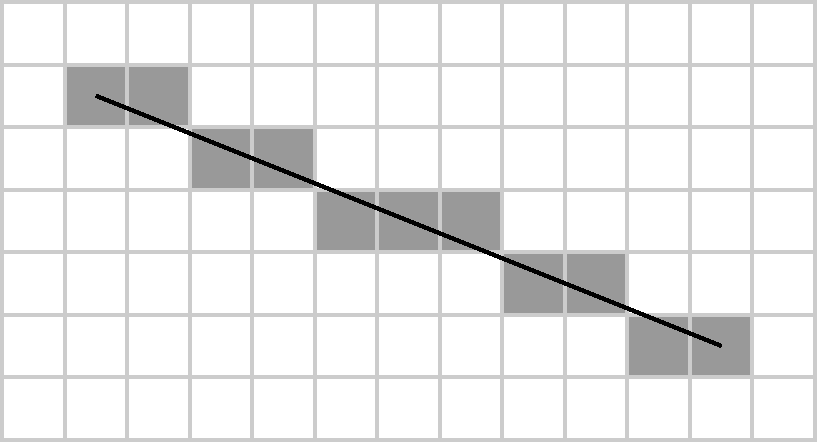
\includegraphics[width=0.33\linewidth]{images/bresenham.pdf}
    \caption{Illustration demonstrating the Bresenham line rendering method.}
    \label{fig:bresenham}
\end{figure}

Since \(A_i \in \mathbb{R^{m^2}}\),  and the maximum number of pixels a line can cover in a matrix of shape \((m, m)\) using the Bresenham algorithm is \(m\), we can conclude that each column has at most \(m\) elements equal to \(1\) and the remaining \(m^2-m\) elements equal to 0. This clearly indicates that sparse matrix representations are ideal for this problem. By using sparse matrices, the computation time is reduced to \(3\) seconds and memory usage drops to \(78MB\), resulting in a significant performance improvement.

\begin{figure}[H]
    \centering
    \begin{minipage}{0.2\linewidth}
        \centering
        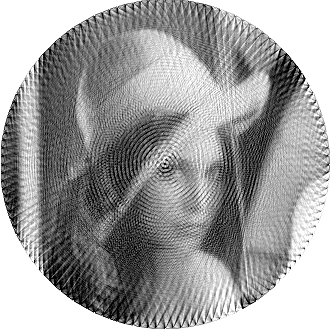
\includegraphics[width=\linewidth]{images/ls/ls_dense.png}
    \end{minipage}
    \begin{minipage}{0.2\linewidth}
        \centering
        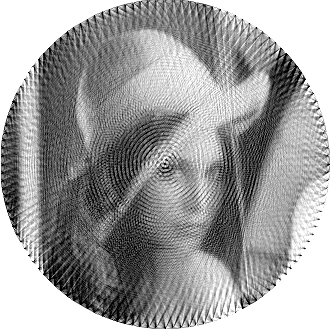
\includegraphics[width=\linewidth]{images/ls/ls_sparse.png}
    \end{minipage}
    \caption{Least Squares results for a system with 128 pegs with dense matrix representation (left) and sparse (right).}
    \label{fig:ls_output}
\end{figure}

\section{Linear Least Squares (LLS)}

To binarize the resulting vector \(x \in \left[-\infty, \infty\right]^{n}\), from the LS solver, a naive approach would be to select the top \(k\) highest values of \(x\) and choose the corresponding lines. To illustrate the limitations of this method, we present three configurations where the top 1000 lines are selected.

\begin{figure}[!htb]
    \centering
    \begin{minipage}{0.32\linewidth}
        \centering
        
\includegraphics[width=\linewidth]{images/ls_binary/ls_rounding.png}
        \caption{Naive binarization of LS solver output.}
        \label{fig:ls_binary}
    \end{minipage}
    \hfill
    \begin{minipage}{0.32\linewidth}
        \centering
        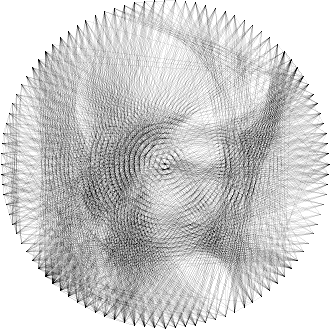
\includegraphics[width=\linewidth]{images/ls_binary/lls.png}
        \caption{Linear Least Squares (LLS) solver.}
        \label{fig:lls}
    \end{minipage}
    \hfill
    \begin{minipage}{0.32\linewidth}
        \centering
        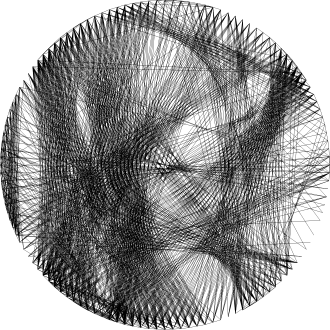
\includegraphics[width=\linewidth]{images/ls_binary/lls_binary.png}
        \caption{LLS solver with binarization and supersampling (\(\sigma=4\)).}
        \label{fig:lls_binary}
    \end{minipage}
\end{figure}

The figures above show the result of the standard LS solver (left), the Linear Least Squares (LLS) solver with box constraints \(x \in \left[0, 1\right]^{n}\) (center), and the LLS solver with both box constraints and binarization using supersampling with \(\sigma = 4\) (right). While the LLS solver requires approximately 30 seconds to compute, this added time is negligible within our scope.

The reason the LS solution (left) tends to select lines along the edge of the circle is due to the possibility of negative coefficients \(x_i\), which effectively allows it to \textit{subtract lines}, analogous to drawing with white string on the canvas. In its attempt to minimize reconstruction error, the solver chooses highly overlapping lines at the edge of the circle so it can subtract from them where needed.

\section{\texorpdfstring{Tuning N and $\sigma$}{Tuning N and sigma}}

The objective of this experiment is to determine the optimal number of pegs \(N\) and the block size \(\sigma\) for generating string art.

For the LS solver, the more we increase the number of pegs, the more the reconstructed image resembles the input image and the lower the residual becomes. However, increasing the number of pegs beyond \(256\) yields only marginal improvements that may not justify the added complexity.

\begin{figure}[H]
    \centering
    \begin{minipage}{0.75\linewidth}
        \centering
        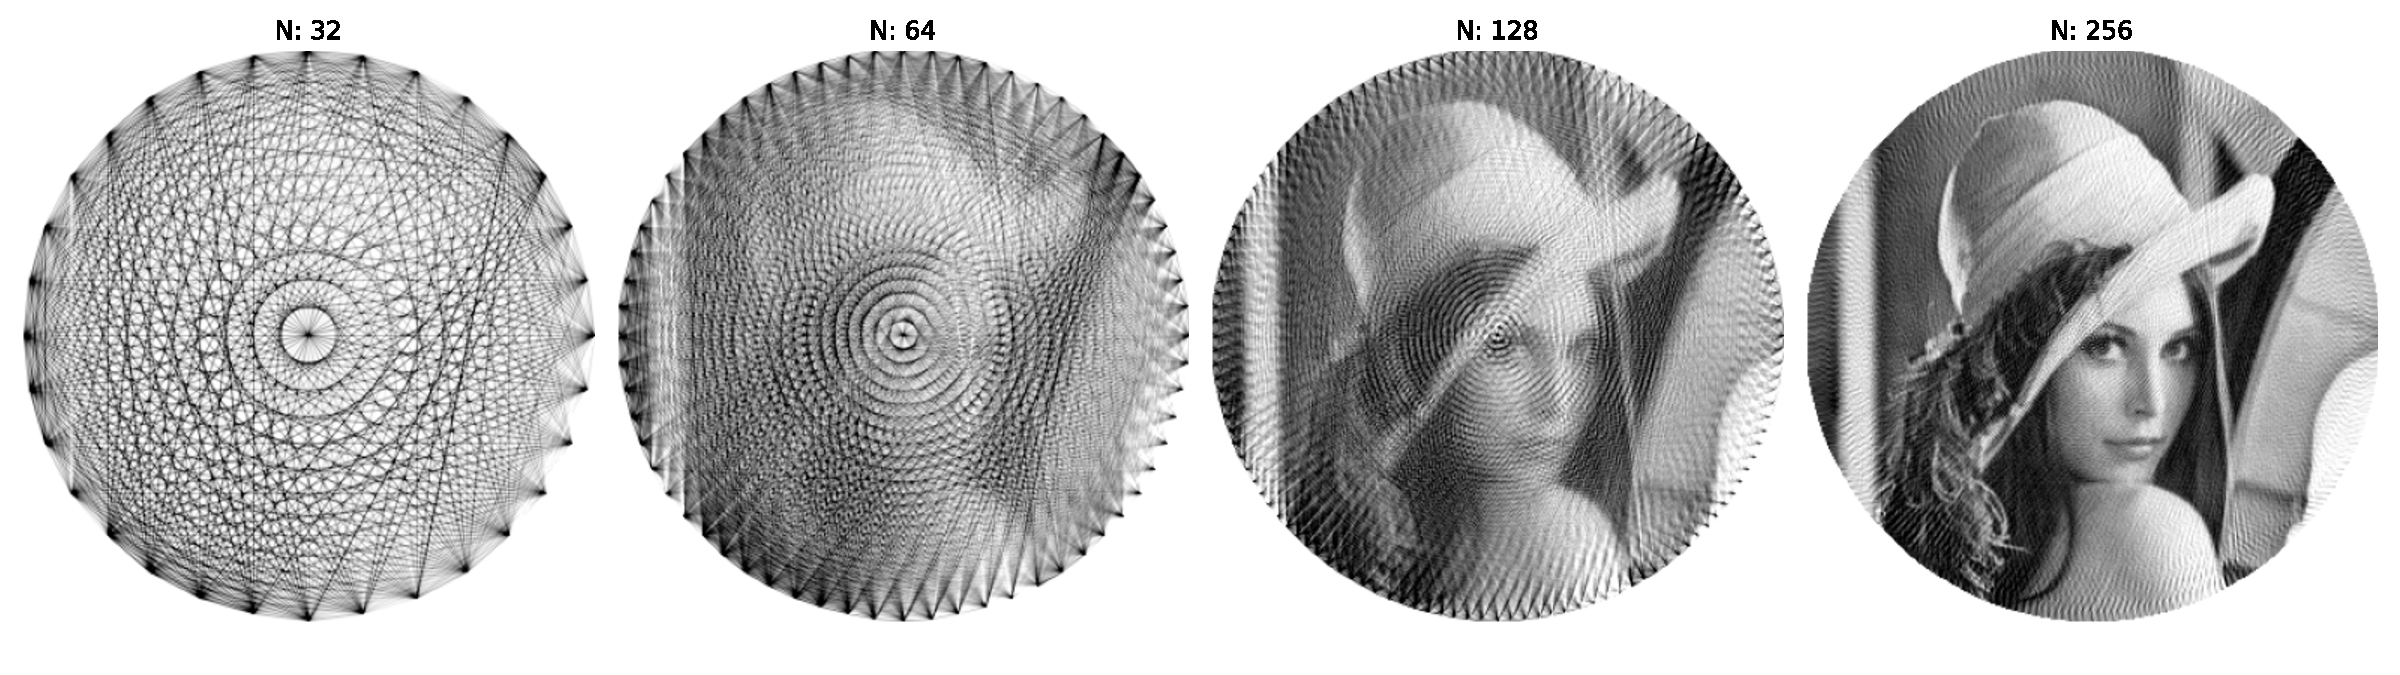
\includegraphics[width=\linewidth]{images/tuning/ls_images.pdf}
    \end{minipage}%
    \hfill
    \begin{minipage}{0.23\linewidth}
        \centering
        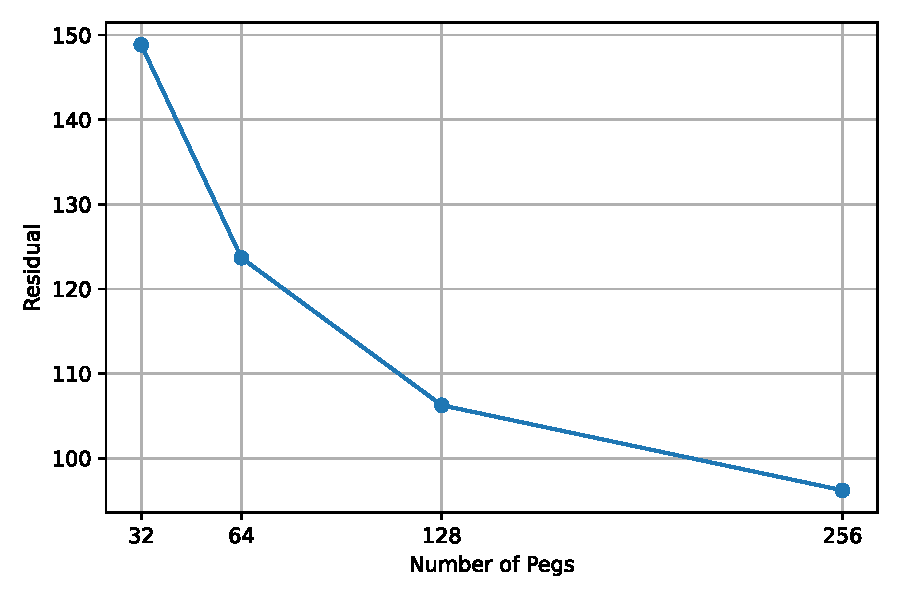
\includegraphics[width=\linewidth]{images/tuning/ls_residuals.pdf}
    \end{minipage}
    \caption{Comparative analysis and plot of residuals for results obtained using LS with different values of \(N\).}
    \label{fig:ls_n_tuning}
\end{figure}

To study the effect of block size \(\sigma\), we switch to a binary solver. This is essential because when we compute at a larger resolution as stated in Supersampling \ref{sec:supersampling}, white areas (thread gaps) grow more significantly than black areas (thread covered regions), affecting visual quality.

\begin{figure}[H]
    \centering
    \begin{subfigure}[t]{0.51\linewidth}
        \centering
        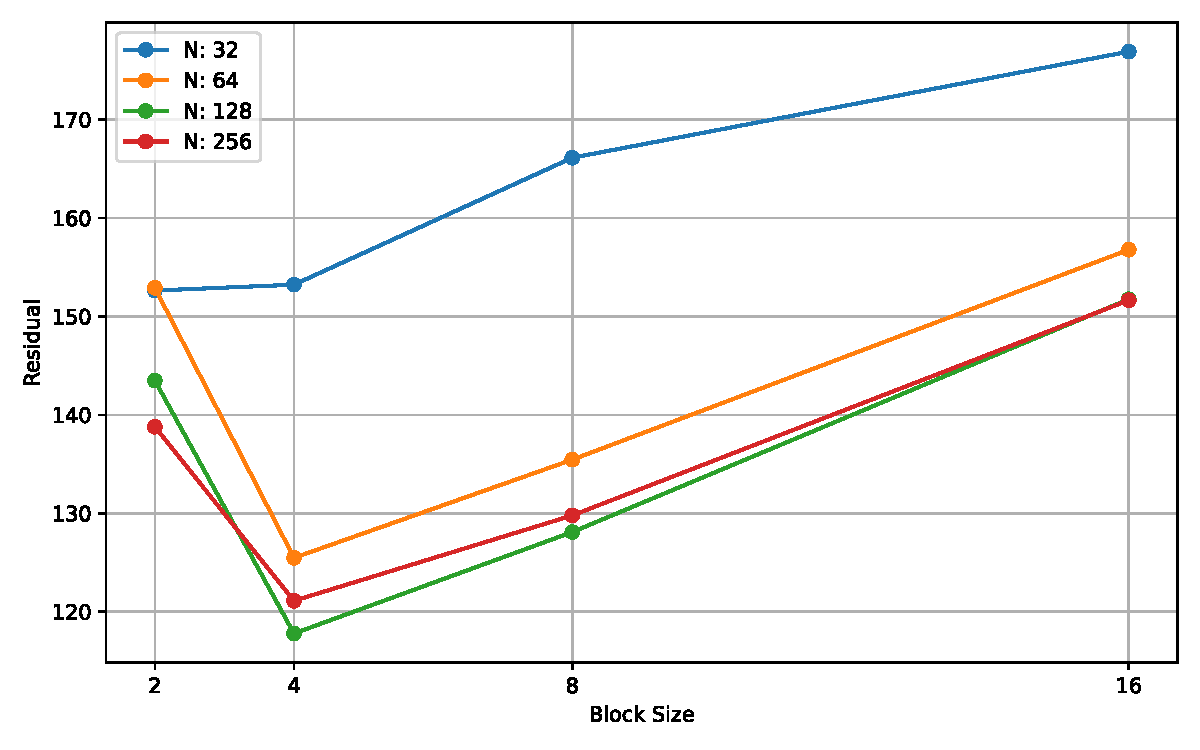
\includegraphics[width=\linewidth]{images/tuning/lls_residuals_by_pegs_and_block_size.pdf}
        \caption{}
    \end{subfigure}%
    \hfill
    \begin{subfigure}[t]{0.33\linewidth}
        \centering
        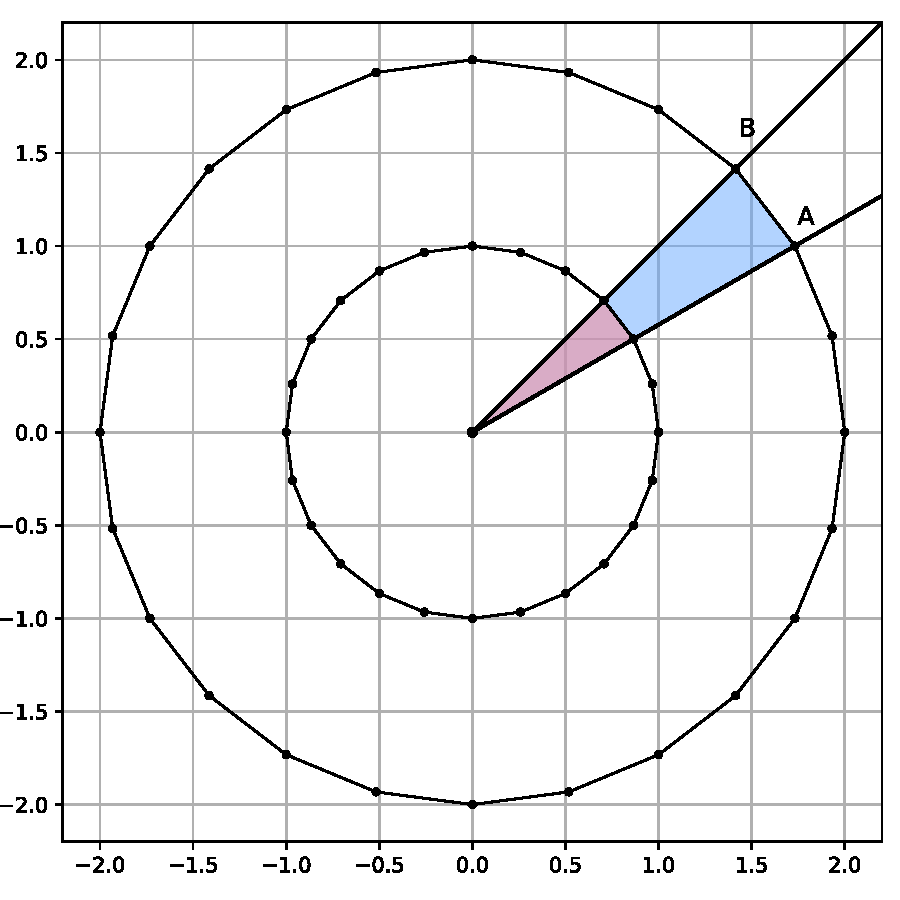
\includegraphics[width=\linewidth]{images/tuning/upsampling.pdf}
        \caption{}
        \label{fig:upsampling_A}
    \end{subfigure}
    \caption{(a) Residual error plotted against block size \(\sigma\). (b) Geometric interpretation of the upsampling process applied to matrix \(A\).}
    \label{fig:lss_residuals_by_pegs_ds}
\end{figure}

\begin{figure}[H]
    \centering
    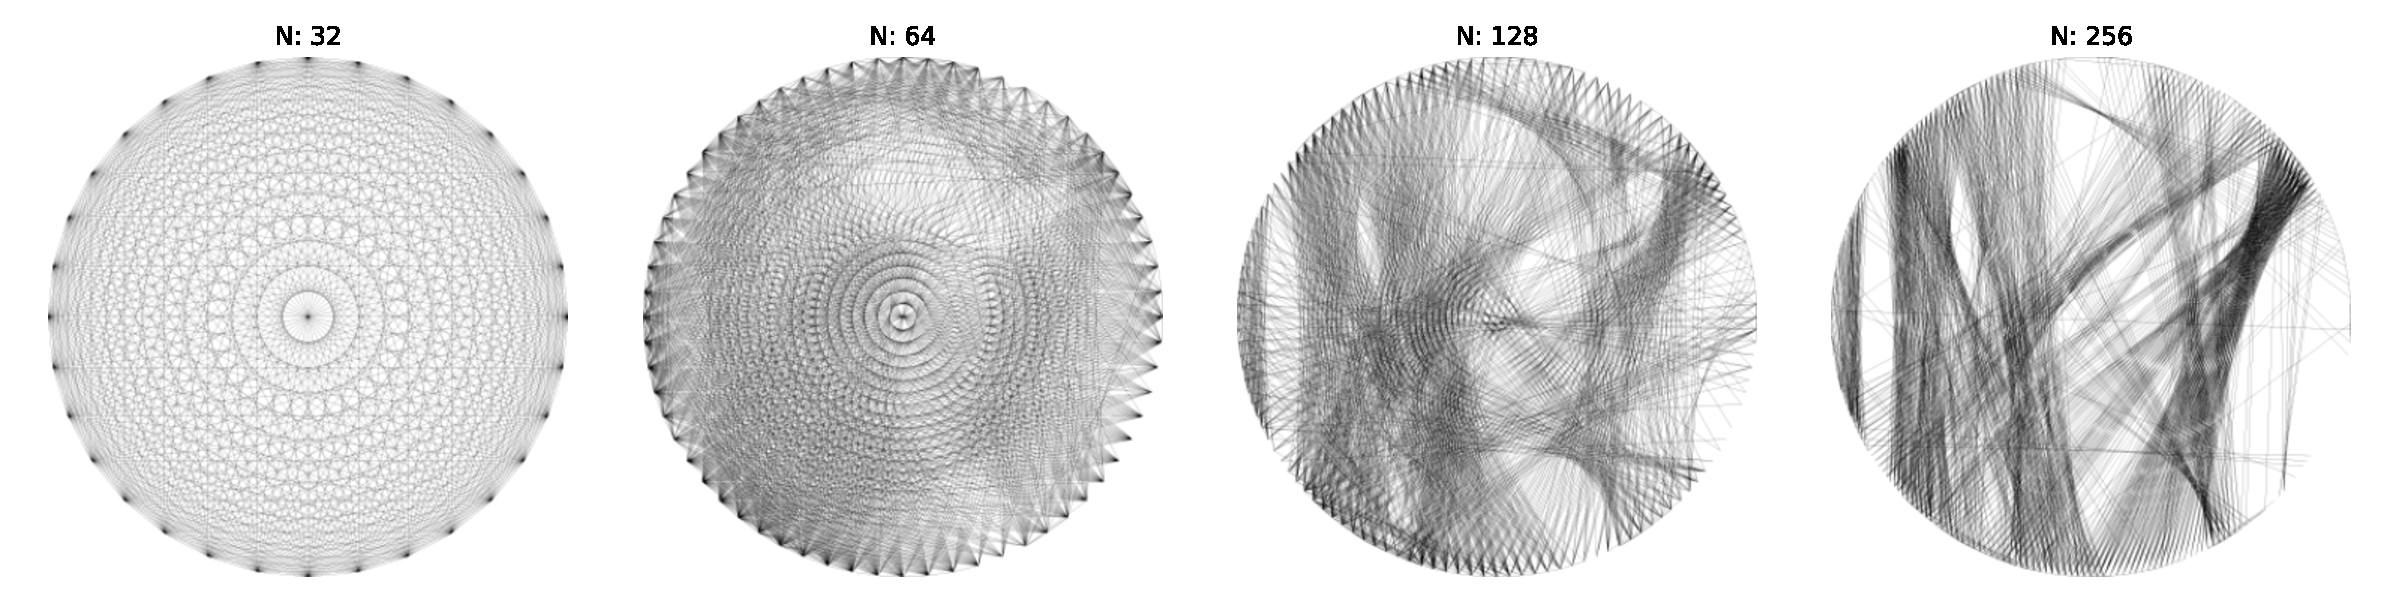
\includegraphics[width=\linewidth]{images/tuning/lls_column_2_as_row.pdf}
    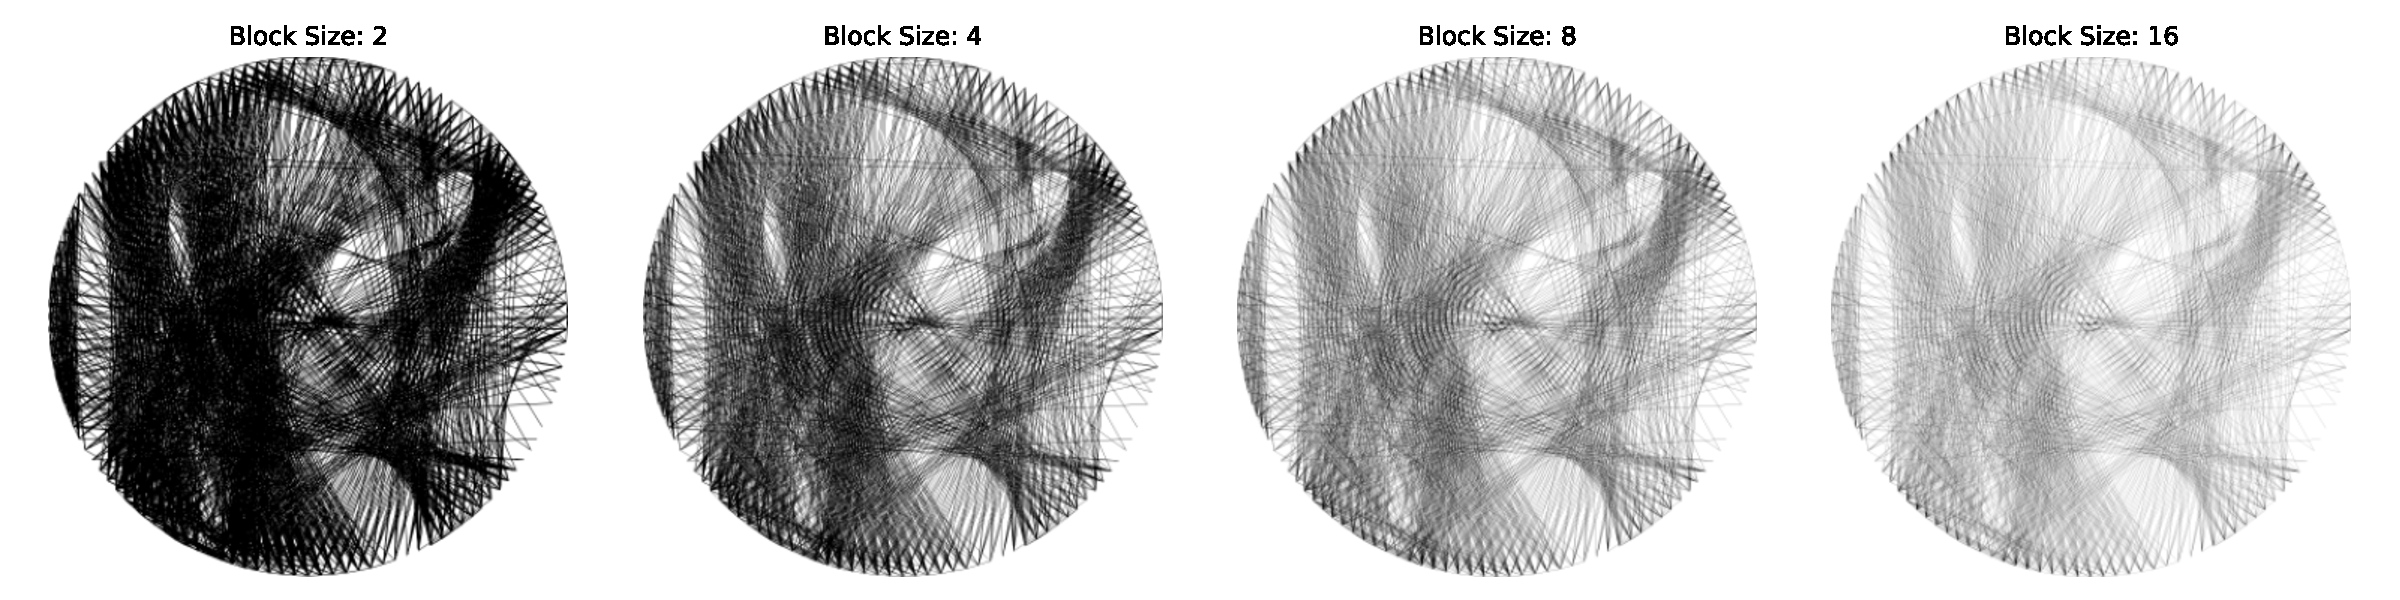
\includegraphics[width=\linewidth]{images/tuning/lls_row_2.pdf}
    \caption{Comparative analysis for varying \(N\) (top) and varying \(\sigma\) (bottom).}
    \label{fig:n_sigma_tuning}
\end{figure}

We can observe in Figure~\ref{fig:n_sigma_tuning} that the block size controls the thread thickness. Increasing it makes the image more transparent. Additionally, for this method, increasing \(N\) too much leads to incorrectly selecting the best lines (due to the naive solution). However, we shouldn't aim to use the maximum number of pegs, but rather choose the most optimal number for the given image. And that raises the question: \enquote{What is the best \(N\) for an image of size \(m \times m\)?}

As we can see in Figure~\ref{fig:upsampling_A}, the inner circle represents the original low-resolution matrix \(A\), while the outer circle corresponds to the upsampled matrix \(\bar{A}\). The white area between two adjacent pegs increases proportionally with the distance between those pegs. The idea is to plot the Manhattan distance and residual error for a selected set of \(N\) values, \(S = \{n_1, n_2, \ldots, n_t\}\), identify the optimal distance, and then use it to derive a formula for a general use. This leads us to:

\[
d = \frac{w}{2}\bigg(\left| \cos(\frac{2\pi}{N}) - 1 \right| + \left|  \sin(\frac{2\pi}{N})\right|\bigg)
\]

where \(w\) is the width of the input image and \(d\) is the manhattan distance between two adjacent pegs (see Appendix~\ref{app:d} for a step-by-step derivation). 

\begin{figure}[H]
    \centering
    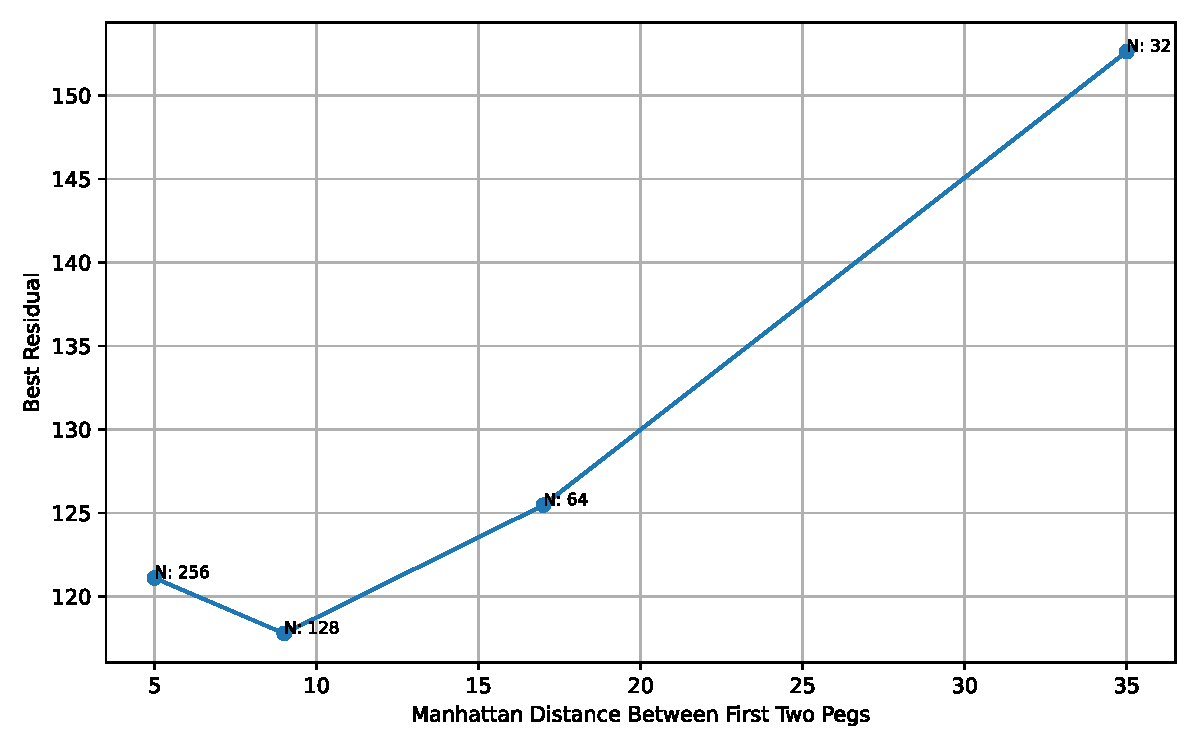
\includegraphics[width=0.5\linewidth]{images/tuning/lls_residuals_by_manhattan_distance.pdf}
    \caption{Best Residual vs. Peg-to-Peg Manhattan Distance.}
    \label{fig:residual_vs_manhattan}
\end{figure}

Plotting \(d\) alongside the residual error yields the figure above, from which we can observe that a Manhattan distance of approximately \(10\) provides the best result. This gives us the final formula:

\[
N = \underset{n \in S}{\arg\min} \left| d(n) - 10 \right|
\]

\section{Least Squares Regularized (LSR)}
\label{sec:lsr}

As explained in Convex Optimization \cite{convex-optimization}, Chapter 4.4, we can cast our problem as a quadratic optimization problem. By using the CVXOPT Python package \footnote{For more details, see \href{https://cvxopt.org/}{CVXOPT: Python Software for Convex Optimization}}, we can integrate constraints and regularization terms. The equation we now need to minimize takes the form of a quadratic problem:

\begin{equation}
\label{eq:qp}
\min_{x} \frac{1}{2} x^TPx + q^Tx \quad \text{subject to } Gx \leq h
\end{equation}

where

\[
P = 2A^\top A, \quad q = -2A^\top b,
\]
\[
G = \begin{bmatrix}
-I \\
I
\end{bmatrix}, \quad
h = \begin{bmatrix}
\mathbf{0} \\
\mathbf{1}
\end{bmatrix}
\]

The constraint \( Gx \leq h \) enforces the box constraint: \(0 \leq x \leq 1\).

\subsubsection{Smooth Regularization}

We now implement the smooth regularization, given by the formula: \(4x(1-x)\). This regularizer promotes binary values by penalizing intermediate values in the range \(\left[0, 1\right]\). While this appears ideal, it has a significant drawback: the function is concave (see Figure~\ref{fig:regularization}), which violates the convexity required for our optimization problem.

To ensure the the matrix \(P\) stays positive semidefinite, a requirement for the CVXOPT solver, a safeguard is implemented by setting the regularization coefficient \(\lambda\) to the lowest eigenvalue of \(P\). Specifically, we ensure: \(\lambda \leq \frac{\lambda_{min}(P)}{8}\). The final modified objective:

\begin{equation}
\label{eq:qp_smooth}
\min_{x} \frac{1}{2} x^T(P - 8 \lambda I)x + (q + 4\lambda1)^Tx \quad \text{subject to } x \in [0,1]^n
\end{equation}

\begin{figure}[H]
    \centering
    \begin{minipage}{0.49\linewidth}
        \centering
        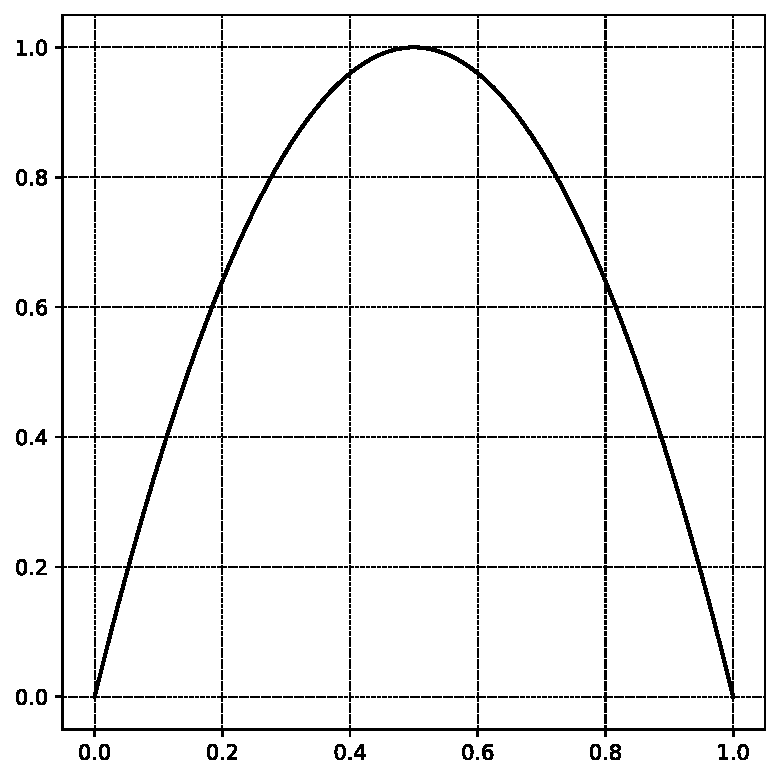
\includegraphics[width=\linewidth]{images/regularization/smooth_regularizer_graph.pdf}
    \end{minipage}%
    \begin{minipage}{0.49\linewidth}
        \centering
        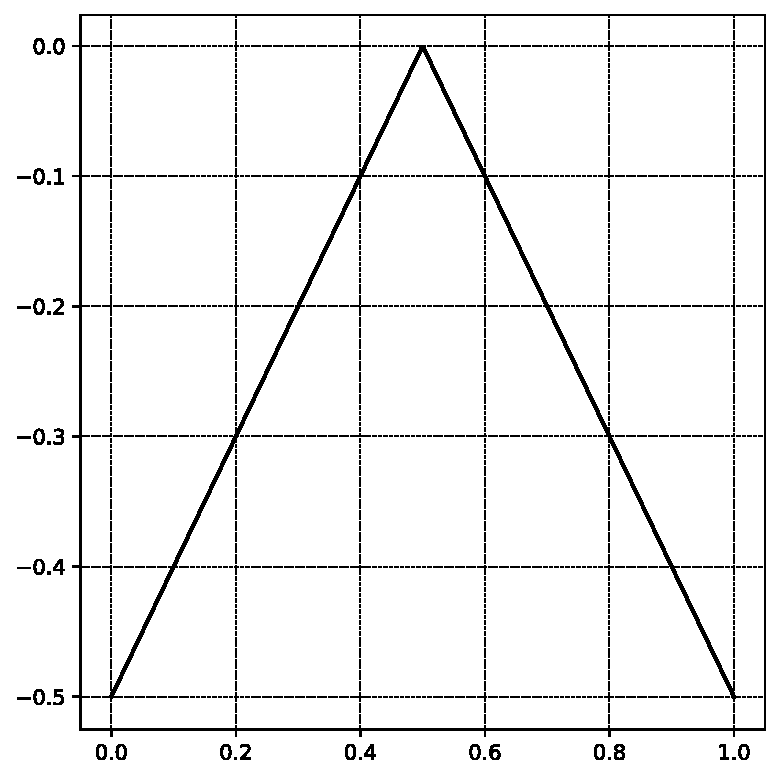
\includegraphics[width=\linewidth]{images/regularization/abs_regularizer_graph.pdf}
    \end{minipage}
    \caption{Smooth regularization graph (left) and Absolute regularization graph (right).}
    \label{fig:regularization}
\end{figure}

\subsubsection{Absolute Regularization}

We now introduce an alternative regularization term, given by the formula: \(1-2\left|x-0.5\right|\), which simplifies to \(-\left|x-0.5\right|\). The term \(\left|x-0.5\right|\) is convex, but its negation is concave. Including it in the objective breaks the convexity of the quadratic problem, making the problem non-convex.

To express the absolute value in a quadratic program, I introduce auxiliary variables: \(t_i \geq \left|x_i - 0.5\right|\) and optimize over: \(z = \left[x;t\right] \in \mathbb{R}^{2n}\). The modified objective and constraints:

\begin{equation}
\min_{x, t} \frac{1}{2} x^TPx + q^Tx - \lambda \sum_i{t_i} \quad \text{subject to } x \in [0,1]^n
\end{equation}

where
\[t \geq x - 0.5, \quad t \geq -x + 0.5\]

\begin{figure}[H]
    \centering
    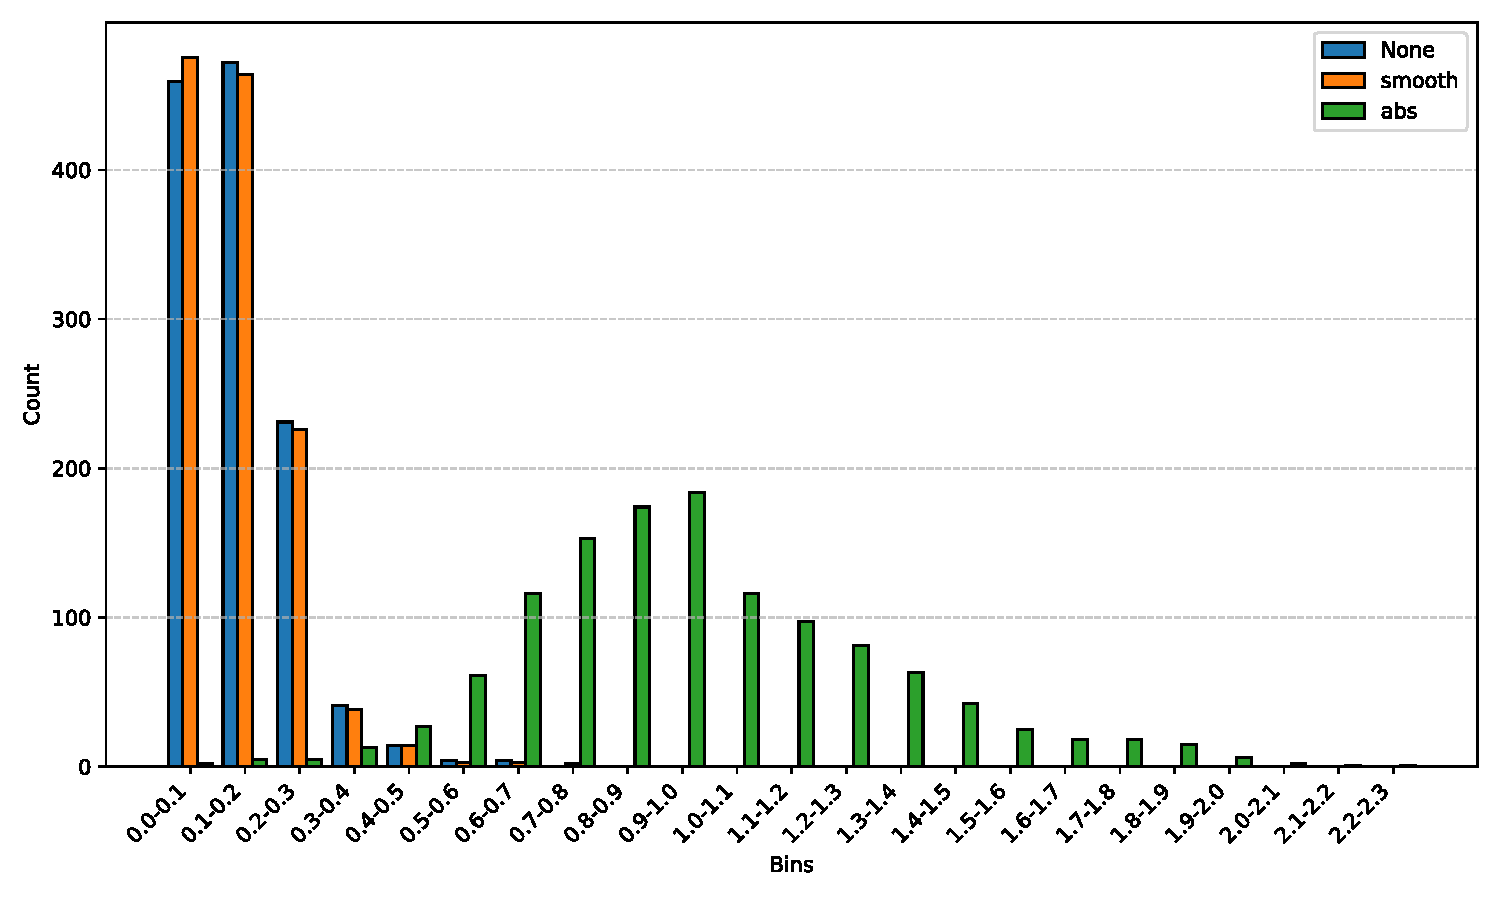
\includegraphics[width=\linewidth]{images/regularization/regularized_x_binned.pdf}
    \caption{Histogram illustrating the distribution of \(x\) coefficients with \(0.1\) bin span.}
    \label{fig:x_binned}
\end{figure}

The Smooth regularizer closely resembles the behavior of having no regularization, that is because the regularization strength \(\lambda\) is set very low to preserve the positive semidefinite property, which can be violated by stronger smoothness penalties. In contrast, the Absolute (abs) regularizer does succeed in pushing values towards \(1\), but it requires a very large regularization weight. However, this high value also causes violations of the imposed box constraints.

\begin{figure}[H]
    \centering
    \begin{minipage}{0.2\linewidth}
        \centering
        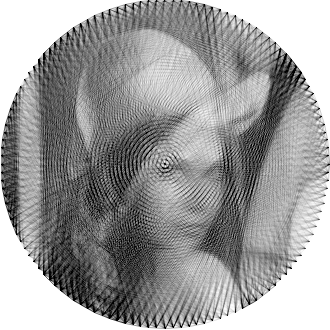
\includegraphics[width=\linewidth]{images/lsr/lsr_smooth.png}
    \end{minipage}
    \begin{minipage}{0.2\linewidth}
        \centering
        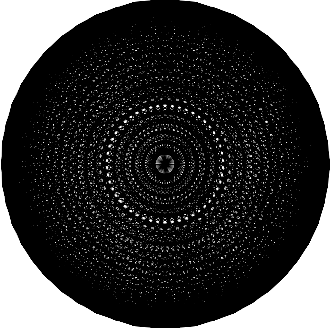
\includegraphics[width=\linewidth]{images/lsr/lsr_abs.png}
    \end{minipage}
    \caption{Least Squares Regularized results for a system with 128 pegs with smooth regularization (left) and absolute (right).}
    \label{fig:lsr_output}
\end{figure}

\section{Binary Projection Least Squares (BPLS)}

In Section~\ref{sec:lsr}, it was noted that introducing a binary enforcing regularization term can break the convexity of the optimization problem. To address this, a new approach was proposed: instead of adding the regularization term explicitly to the objective, we incorporate its effect directly into the cost matrix before solving the system. This preserves convexity while still encouraging binary-like solutions through adaptive weighting.

We will now introduce the following vector \(w\). This vector forms the diagonal of a regularization matrix \(W = diag(w)\), which is used to modify the original quadratic cost matrix \(P\). The updated regularized problem becomes:

\begin{equation}
\label{eq:bpls}
\min_{x} \frac{1}{2} x^T(P + \lambda W)x + q^Tx \text{ subject to } x \in [0,1]^n
\end{equation}

The first iteration begins with \(W = I\), and we update the weights at step \(i\) using the formula \(w_i = x_{i-1}(1-x_{i-1}) + \epsilon\). We solve the problem described by Equation~\ref{eq:bpls}, then select the the top \(k\) values from \(x\) and fix those to \(1\). Next, we adjust the problem by calculating the contributions of the selected lines: \(A_1 \cdot 1\), where \(A_1\) is the subset of lines corresponding to the selected indices in this iteration. We subtract this from \(b\): \(\bar{b} = b - A_1 \cdot 1\). This process is repeated with the updated \(\bar{b}\) until the error stops decreasing or a maximum number of iterations is reached.

\begin{figure}[H]
    \centering
    \begin{minipage}{0.2\linewidth}
        \centering
        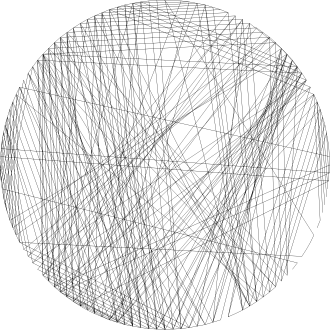
\includegraphics[width=\linewidth]{images/bpls/bpls_earlystopping.png}
    \end{minipage}
    \begin{minipage}{0.2\linewidth}
        \centering
        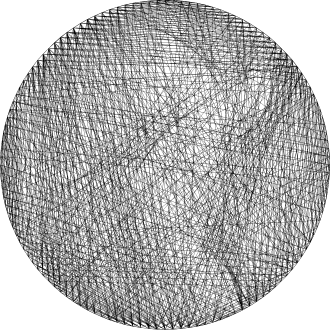
\includegraphics[width=\linewidth]{images/bpls/bpls.png}
    \end{minipage}
    \caption{Binary Projection Least Squares results for a system with 128 pegs and \(k=10\): with early stopping (left) and without early stopping, using a maximum of 90 iterations (right).}
    \label{fig:bpls_output}
\end{figure}

\section{Matching Pursuit (MP)}

Matching Pursuit is a greedy algorithm used to approximate a signal by selecting dictionary vectors one by one. In our case, the signal is the \(b\) vector, and the dictionary vectors are the column vectors of the matrix \(A\).

Below, we present two methods of matching pursuit: Greedy Matching Pursuit and Orthogonal Matching Pursuit (OMP). Both methods will be analyzed using the selection of 1000 lines, with experiments conducted using both real valued and binary coefficients.

\subsection{Greedy}

The greedy method consists of selecting the line the reduces the residual error the most at each step. Once a line is chosen, the decision is irreversible. This method is computationally intensive on a typical personal use PC. To address this, we introduce two heuristics to reduce the number of candidate lines evaluated at each step: random, where we randomly select \(l\) candidate lines, in our experiments \(l=100\) provides a good trade-off between accuracy and computation time, and dot-product, where we compute the scalar product \(A^Tb\) and select the top \(l\) based on this score. See Appendix~\ref{app:greedy} for the pseudocode of this algorithm.

\subsection{Orthogonal Matching Pursuit (OMP)}

The Orthogonal Matching Pursuit (OMP) method is very similar to the Greedy one, following the same kind of iterative process based on selecting the line that reduces the error the most. In contrast, OMP updates the residual \(b\) (initially the input image) by subtracting the projection of the selected line. This ensures that the residual remains orthogonal to all lines selected so far. See Appendix~\ref{app:omp} for the pseudocode of this algorithm.

\begin{figure}[H]
    \centering
    \begin{minipage}{0.2\linewidth}
        \centering
        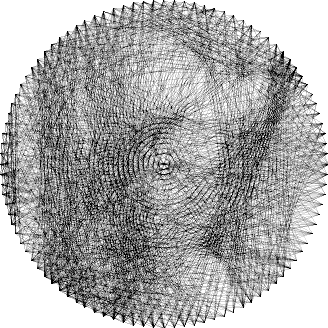
\includegraphics[width=\linewidth]{images/mp/greedy_random.png}
    \end{minipage}
    \begin{minipage}{0.2\linewidth}
        \centering
        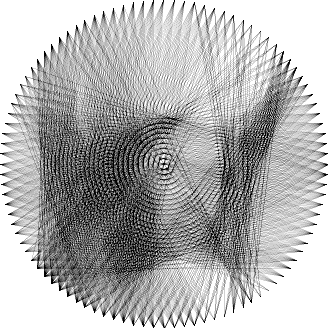
\includegraphics[width=\linewidth]{images/mp/greedy_dotproduct.png}
    \end{minipage}
    \begin{minipage}{0.2\linewidth}
        \centering
        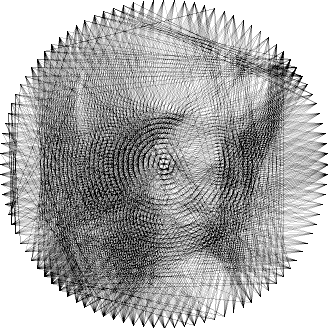
\includegraphics[width=\linewidth]{images/mp/omp.png}
    \end{minipage}
    \caption{Matching Pursuit results for a system with 128 pegs and 1000 selected lines, using real valued \(x\) coefficients and without early stopping. The methods, in order, are: greedy (random heuristic), greedy (dot-product heuristic), and Orthogonal Matching Pursuit.}
    \label{fig:mp_outputs}
\end{figure}

\begin{figure}[H]
    \centering
    \begin{minipage}{0.2\linewidth}
        \centering
        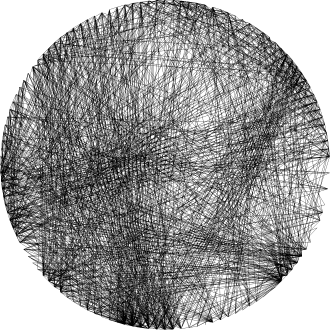
\includegraphics[width=\linewidth]{images/mp_binary/greedy_random_binary.png}
    \end{minipage}
    \begin{minipage}{0.2\linewidth}
        \centering
        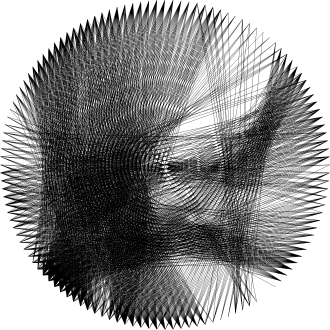
\includegraphics[width=\linewidth]{images/mp_binary/greedy_dot-product_binary.png}
    \end{minipage}
    \begin{minipage}{0.2\linewidth}
        \centering
        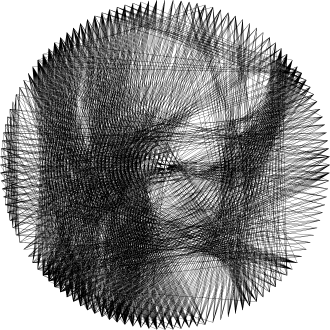
\includegraphics[width=\linewidth]{images/mp_binary/omp_binary.png}
    \end{minipage}
    \caption{Matching Pursuit results for a system with 128 pegs and 1000 selected lines, using binary valued \(x\) coefficients with supersampling and without early stopping. The methods, in order, are: greedy (random heuristic), greedy (dot-product heuristic), and Orthogonal Matching Pursuit.}
    \label{fig:mp_binary_outputs}
\end{figure}

\section{Radon Transform}

The Radon Transform maps an image \(f(x,y)\) to a collection of line integrals through \(f(x,y)\). We can express it as follows: \(\text{Let } L(\theta, s) = \{(x, y) \in \mathbb{R}^2 : x\cos\theta + y\sin\theta = s\} \text{ be the line integral}\), where \(\theta \in \left[0, \pi\right)\) is the angle the line makes with the x-axis and \(s \in \left[ -r, r\right]\), is the signed perpendicular distance from the origin to the line, and \(r\)  is the radius of the inscribed circle within the image. Then, we define:

\begin{equation}  
R(\theta, s) = \int_{L(\theta, s)} f(x, y)ds
\end{equation}

\begin{figure}[H]
    \centering
    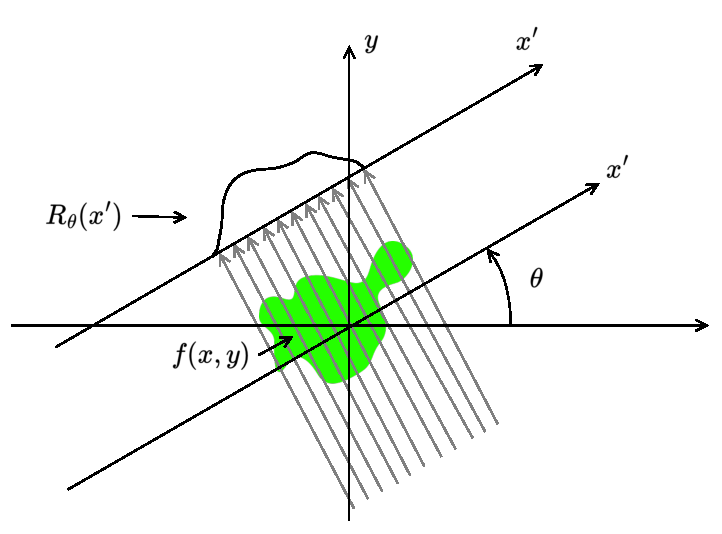
\includegraphics[width=0.6\linewidth]{images/radon.pdf}
    \caption{Radon Transform Illustration.}
    \label{fig:radon_illustration}
\end{figure}

Using the illustration above, we can think of the Radon transform like a laser beam that scans through the image. At each angle and distance, the laser measures how much of the image’s content (or density) it passes through. By collecting these measurements from different angles and positions, we get a full set of line integrals that represent the image from many perspectives.

In our string art problem, the lines we draw can also be described using the same notation with \(\theta\) and \(s\) as above. This means another way to solve the string art problem is to compute the Radon Transform of all possible lines across our circle and select the line with the highest value to draw next. \textbf{Important}: each line’s projection should be normalized by dividing by its length. Otherwise, the algorithm would favor longer lines over shorter, darker ones.

After selecting a line, we need to subtract its contribution from the sinogram, and also from all other lines. Because lines intersect and depend on each other, this means the basis is not orthogonal. We continue this process as long as the error decreases by more than a minimum delta, and we use a customizable patience factor to control when to stop.

We implemented a custom Radon Transform because we can take advantage of the constraints in the string art problem. Instead of representing the sinogram as a matrix indexed by \(\theta\) and \(s\), it’s stored as a list where each index \(i\) corresponds to the density of line \(i\). We select the line with the highest value, remove it from the list, and then update all other lines by removing the pixels that intersect with the chosen line. This keeps the space orthogonal. This update step has time complexity \(O(n^2)\).

\begin{figure}[H]
    \centering
    \begin{minipage}{0.2\linewidth}
        \centering
        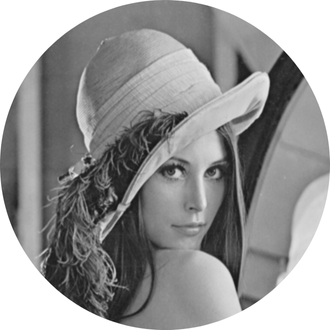
\includegraphics[width=\linewidth]{images/radon/lena_bw.png}
    \end{minipage}
    \begin{minipage}{0.2\linewidth}
        \centering
        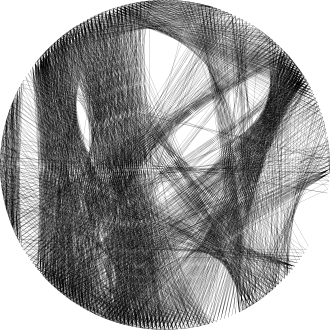
\includegraphics[width=\linewidth]{images/radon/lena_radon.png}
    \end{minipage}
    \begin{minipage}{0.2\linewidth}
        \centering
        \includegraphics[width=\linewidth]{images/radon/mary.png}
    \end{minipage}
    \begin{minipage}{0.2\linewidth}
        \centering
        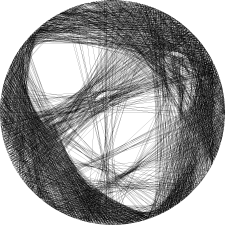
\includegraphics[width=\linewidth]{images/radon/mary_radon.png}
    \end{minipage}
    \caption{Radon Transform results for a system with 256 pegs and early stopping mechanism.}
    \label{fig:radon_output}
\end{figure}

\subsubsection{Enhancing the Radon Transform Method}
\label{sec:radon_improvements}

While standard Radon implementations (like those in scikit-learn) run in \(O(nlogn)\), our approach avoids the overhead of computing the sinogram of the intersection between two lines and then subtracting it from all other lines. Although this may sound straightforward, it is actually more complex than implementing manual projection calculations and the orthogonal projection update.

Another way to speed up our Radon Transform is to update only the lines that intersect the chosen line, limiting updates to the number of intersections instead of all lines. Of course, the initial computation of the Radon Transform still has a time complexity of \(O(n)\). However, when subtracting the contribution of the chosen line, the update step now becomes more efficient, with time complexity \(O(k)\), where \(k\) is the maximum number of possible intersections across all lines. 

This raises an important question: \textit{Which is the worst line to draw?}, or more formally: \textit{Which line causes the most intersections if drawn?} As a result, the final time complexity becomes \(O(nk)\).

To answer the question above, intersections occur when the selected line partitions the circle into two regions, and other lines attempt to connect points from opposite sides of this partition. Any such line will necessarily intersect the dividing line. Intuitively, the worst-case dividing line is the one that perfectly splits the circle into two equal halves. In this case, each of the \(\frac{N}{2}\) pegs on one side can potentially connect to each of the \(\frac{N}{2}\) pegs on the other side, resulting in a maximum of \((\frac{N}{2})^2 = \frac{N^2}{4}\) intersections. This remains to be formally proven.
\chapter{Performance Evaluation and Analysis}

\section{Experiment Setup}

In Figure~\ref{fig:diff_images} we ran different solvers on the same input image to compare them visually, as well as in terms of time and memory efficiency. All solvers used the same image preprocessing and the same drawing algorithm (Xiaolin-Wu). Solvers (a) through (h) used 128 pegs, while solver (i) used 256. Increasing the number of pegs for all solvers either results in incorrect line selection (due to naive line selection methods) or significantly higher computation time.

Solver (a) uses least squares with real coefficients. Solver (b) is a binary rounding of (a), using the top 1000 lines selected based on the coefficients from (a). Solver (c) constrains coefficients to lie within \(\left[0, 1\right]\) and selects 1000 lines. Solver (d) is a binarization of (c), using supersampling with \(\sigma=4\).

Solver (e) is a regularized version of least squares. Solver (f) is binary projection least squares. Solvers (g) and (h) both use orthogonal matching pursuit with 1000 line selections: (g) with real coefficients and (h) in binary form, the latter employing supersampling with \(\sigma=4\).

Finally, solver (i) is the Radon solver, which allows unlimited lines but includes an early stopping mechanism and uses \(\sigma=8\)

\section{Benchmarks}

\begin{table}[!ht]
\centering
\caption{Computation Time, Peak Memory Usage, and RMS of Different Solvers}
\begin{tabularx}{\textwidth}{l C C C}
\toprule
\textbf{Solver} & \textbf{Computation Time (s)} & \textbf{Peak Memory Usage (MB)} & \textbf{RMS} \\
\midrule
(a) ls     &    32.531          &   \textbf{321.970} & 0.1530          \\
(b) ls     &    \textbf{31.640} &   \textbf{321.970} & 0.2933          \\
(c) lls    &   169.719          &   770.275          & 0.3243          \\
(d) lls    &   172.250          &   770.273          & 0.2255          \\
(e) lsr    &   324.468          &  9596.899          & \textbf{0.1488} \\
(f) bpls   & 14499.700          & 10112.366          & 0.4447          \\
(g) mp     &    59.464          &  2762.394          & 0.2427          \\
(h) mp     &   158.776          &  1242.166          & 0.2339          \\
(i) radon  &  2170.854          &  1255.895          & 0.1807          \\
\bottomrule
\end{tabularx}
\end{table}

\begin{figure}[H]
    \centering
    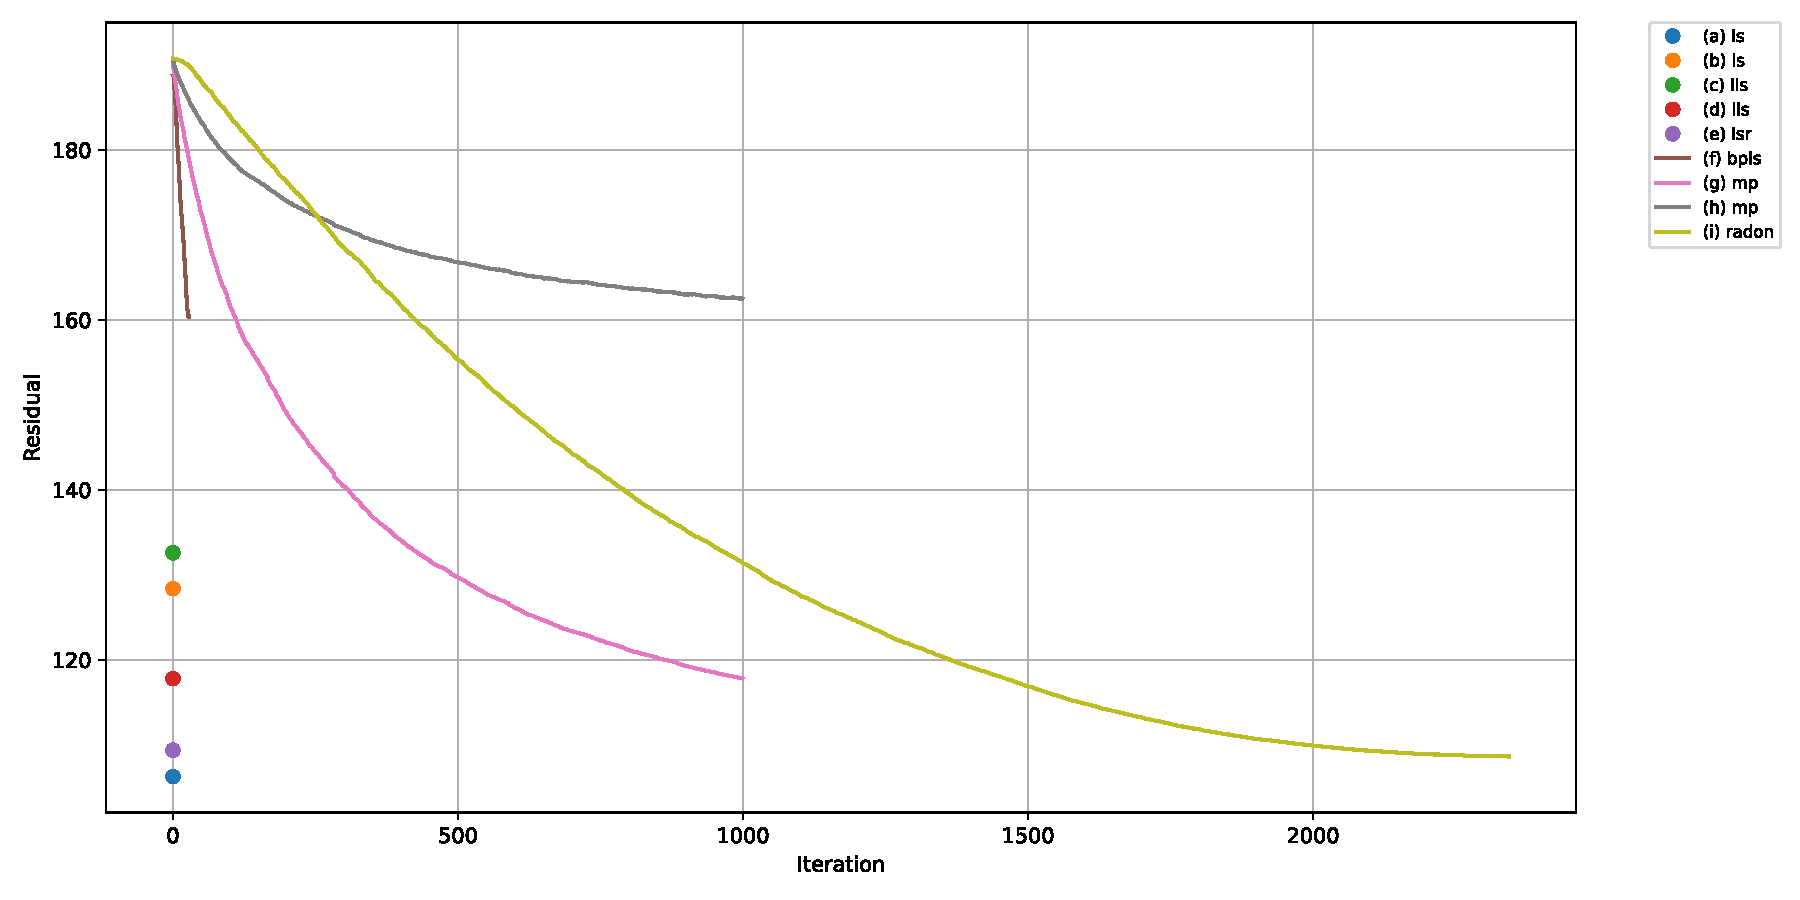
\includegraphics[width=\linewidth]{images/benchmarks/residual_history.pdf}
    \caption{Residual error over iterations for each solver.}
    \label{fig:residual_history}
\end{figure}

\section{Evaluation Summary}

The lowest RMS value belongs to (e) lsr, however, it is very close to (a) ls while being 10× slower and consuming 30× more memory. The RMS delta is negligible (\(\approx\)0.0042). Being the simplest, the (a) ls solver is both the fastest and the most memory efficient. However, its visual output is not desirable, we would prefer our best choice to be a binary solver. This narrows the candidates to (d), (f), (h), or (i). Among these, the best subjective image quality belongs to (d) LLS, while the best RMS score is achieved by (i) radon. One advantage of (i) radon is its ability to separate the subject from the background: the white areas are more prominent, and the overall line selection pattern appears more organized.

Looking at Figure~\ref{fig:residual_history}, we observe that (i) shows a slow, steady decrease in residuals. Other solvers, like (f), drop more aggressively, but this doesn’t necessarily yield better visual results. Among the iterative methods, (i) is the most stable and achieves the lowest residual error. Given these observations, along with its reasonable time and memory usage, we conclude it offers the best overall balance. To confirm this further, we compare it on another image:

\begin{figure}[H]
    \centering
    \begin{minipage}{0.2\linewidth}
        \centering
        \includegraphics[width=\linewidth]{images/lls vs radon/mary.png}
    \end{minipage}
    \begin{minipage}{0.2\linewidth}
        \centering
        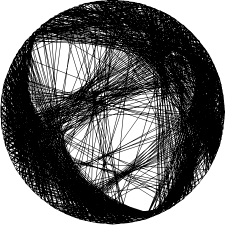
\includegraphics[width=\linewidth]{images/lls vs radon/lls.png}
    \end{minipage}
    \begin{minipage}{0.2\linewidth}
        \centering
        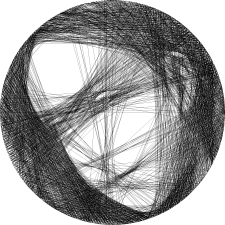
\includegraphics[width=\linewidth]{images/lls vs radon/radon.png}
    \end{minipage}
    \caption{Comparative analysis between (d) lls (center) and (i) radon (right), with input image (left).}
    \label{fig:lls_vs_radon}
\end{figure}

\begin{figure}[H]
    \centering
    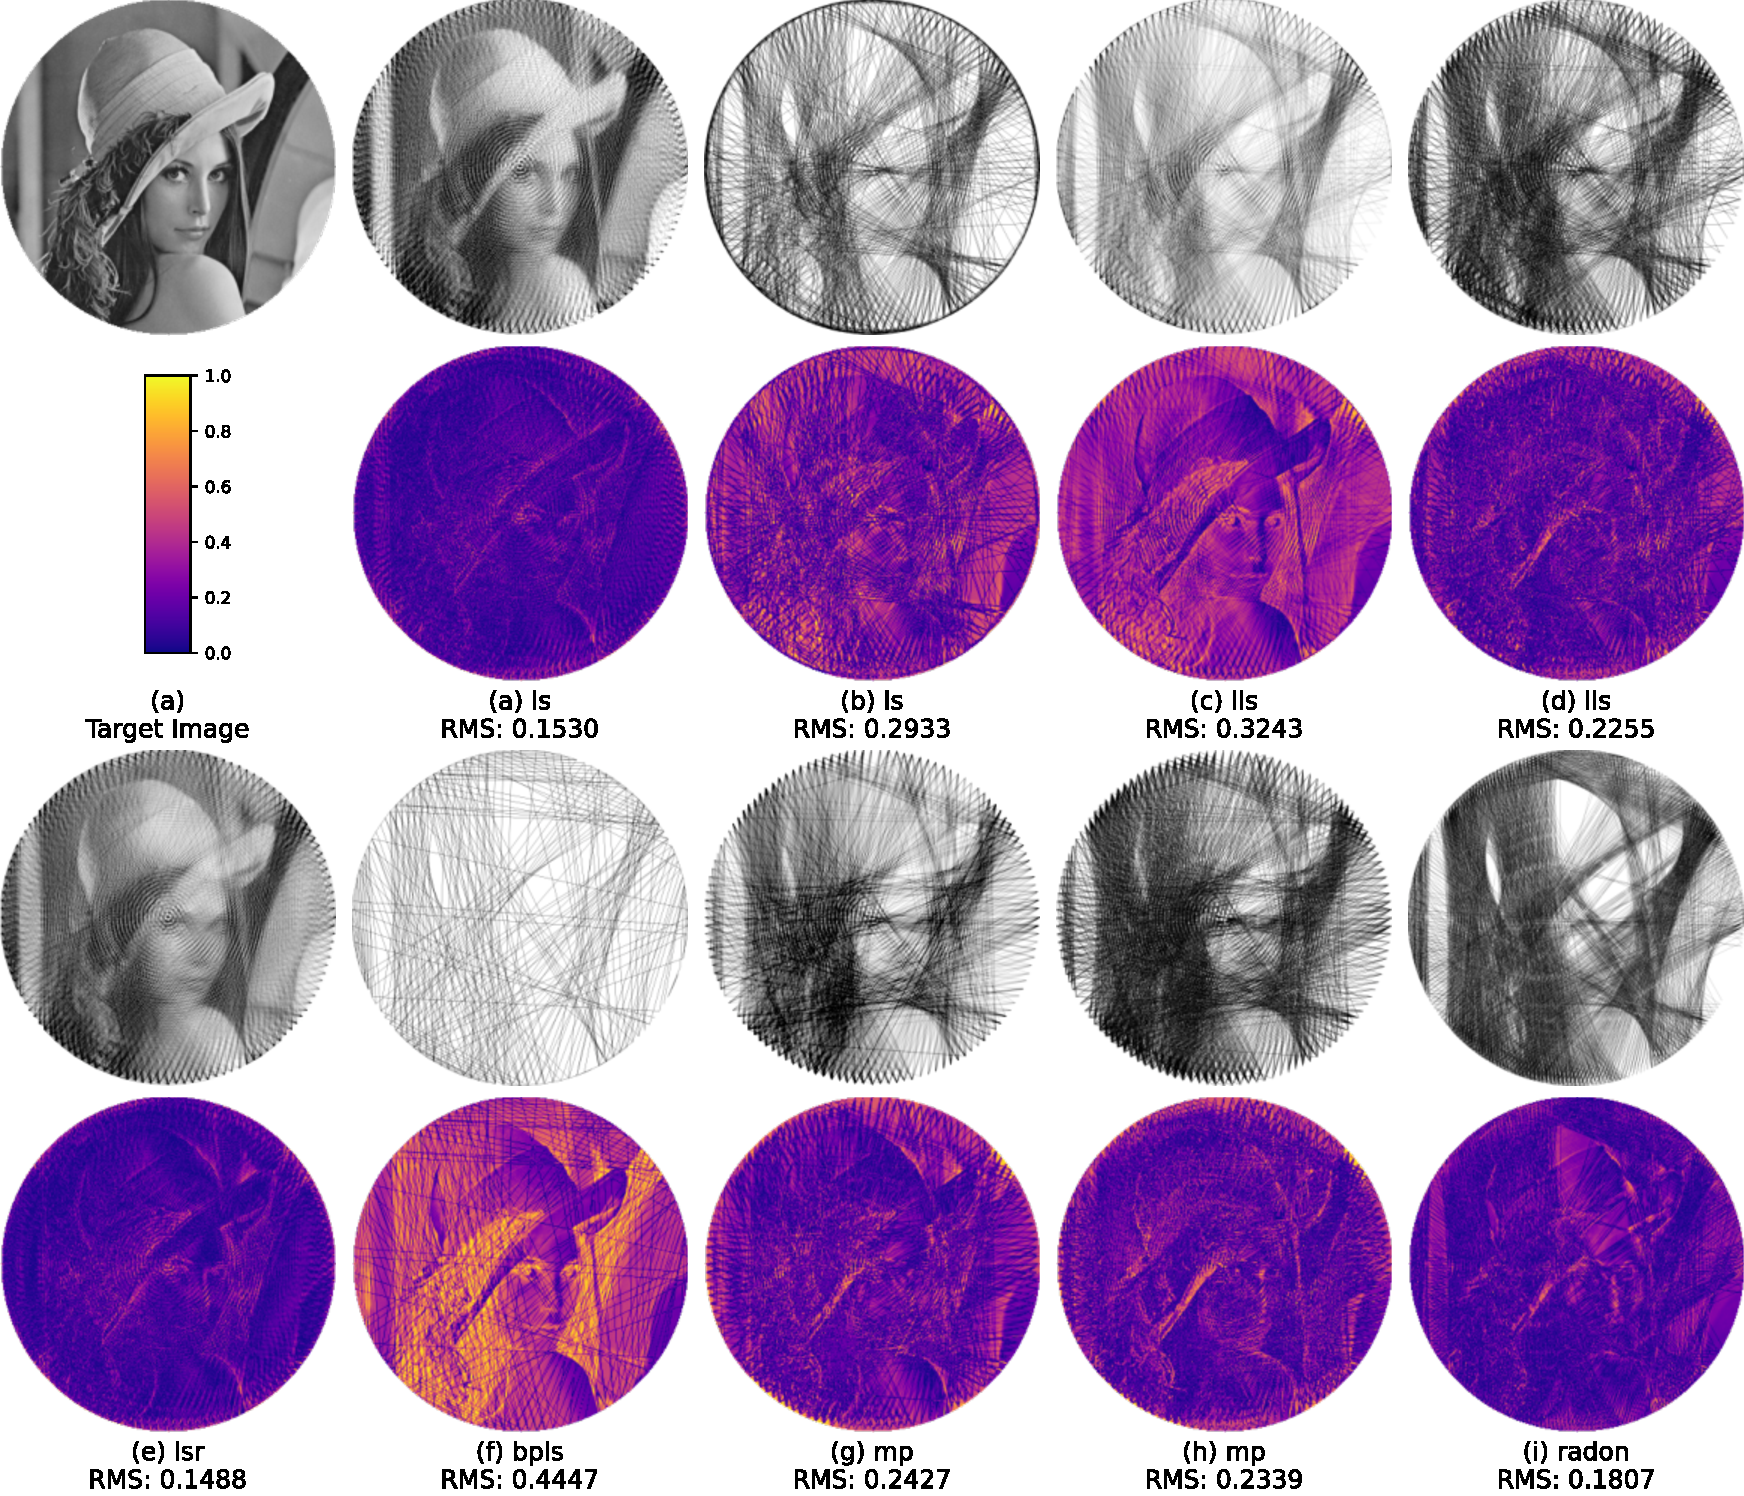
\includegraphics[width=0.9\linewidth]{images/benchmarks/diff_images.pdf}
    \caption{Comparative analysis of the results produced by different solvers. The first image is the input target image, and for each solver, we display the reconstructed image alongside the absolute difference image with respect to the target.}
    \label{fig:diff_images}
\end{figure}

\chapter{Summary and Outlook}

\subsubsection{Conclusion}

In this thesis, we analyzed several optimization algorithms for the radial reconstruction of images  with a focus on the string art problem. We examined the strengths and weaknesses of each, tuned parameters, and proposed and implemented a new method using the Radon Transform. Our analysis and benchmarks conclude that this approach offers the best balance of reconstruction quality, time and memory efficiency, and stability. For additional tests and detailed results, please refer to Appendix~\ref{app:radon_quantitative}.

\subsubsection{Future work}

In future work, we plan to implement the enhancements to the Radon Transform described in Section~\ref{sec:radon_improvements}. 

Following the modern trend of applying deep learning to classical problems, we experimented with a custom Generative Adversarial Network (GAN) featuring a simplified UNet generator and a custom discriminator to achieve style transfer of string art from normal images. See the results in Figure~\ref{fig:ai}. The code is publicly available at \href{https://github.com/skpha13/stringnet}{stringnet}.

\begin{figure}[H]
    \centering
    \begin{minipage}{0.7\linewidth}
        \centering
        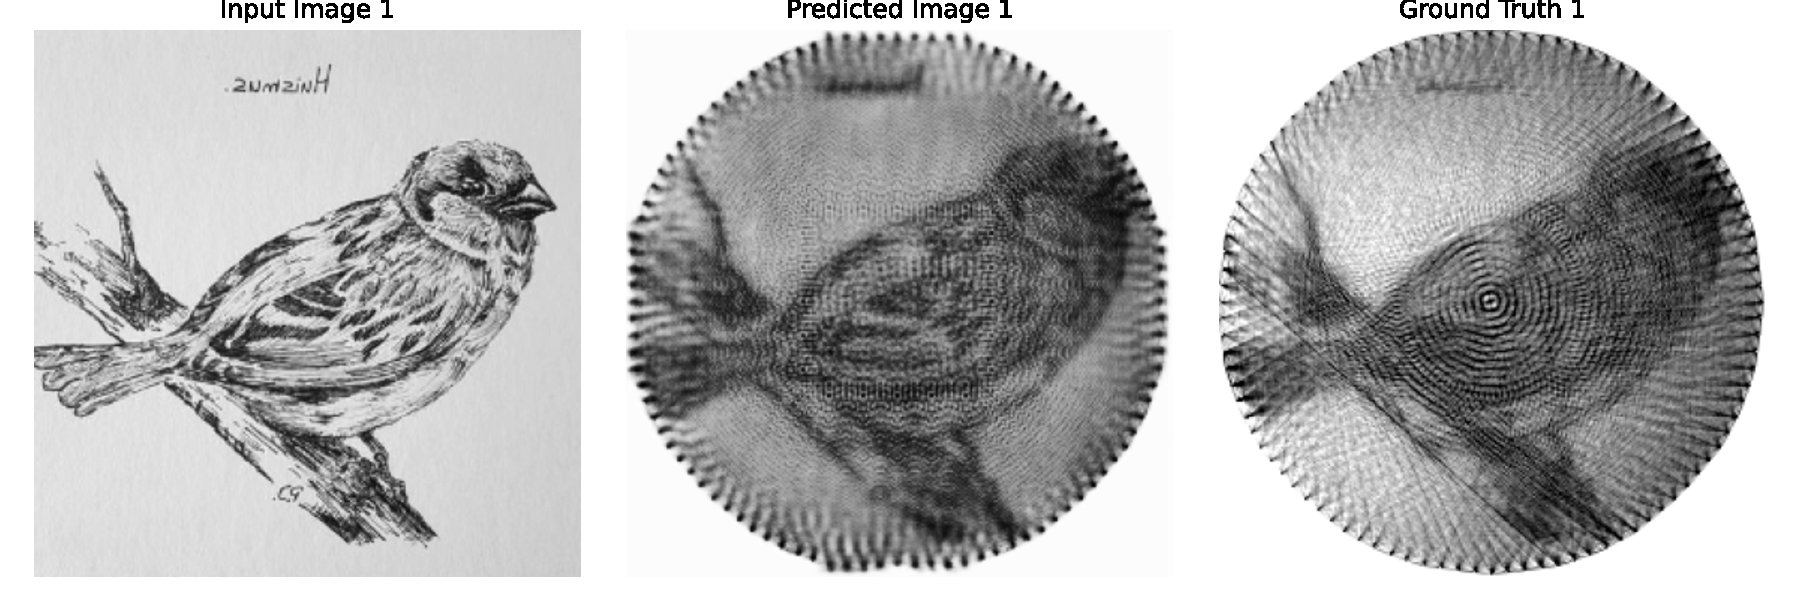
\includegraphics[width=\linewidth]{images/AI/predictions.pdf}
    \end{minipage}%
    \hfill
    \begin{minipage}{0.3\linewidth}
        \centering
        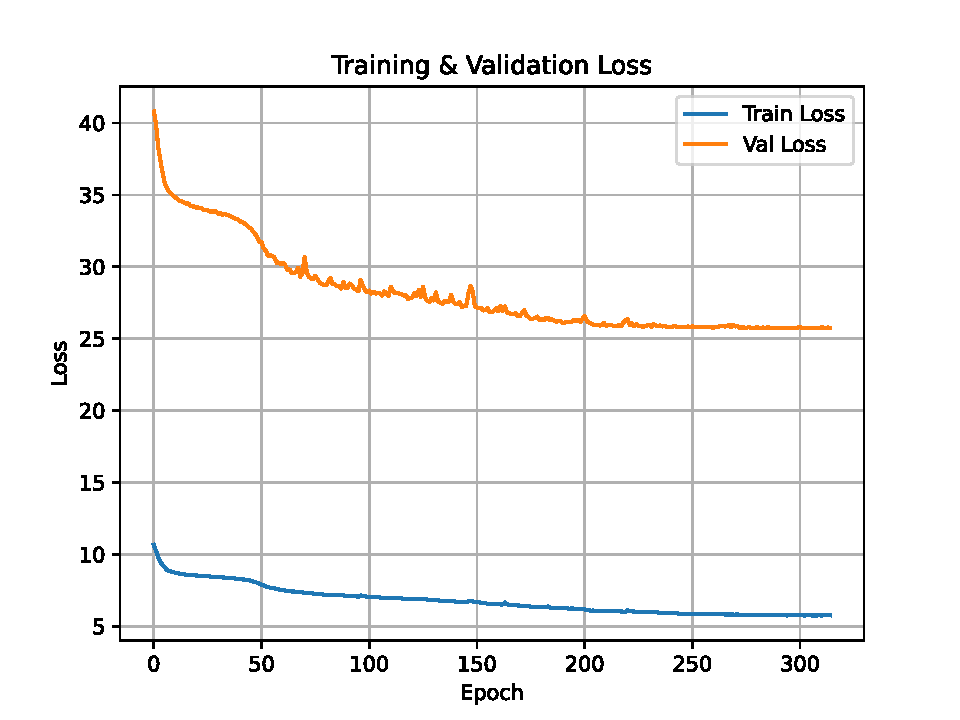
\includegraphics[width=\linewidth]{images/AI/loss.pdf}
    \end{minipage}
    \caption{Results of Generative Adversarial Network for string art image style transfer.}
    \label{fig:ai}
\end{figure}

The idea above works as style transfer, but we could set a fixed number of pegs and then use a deep learning algorithm to find the activation of lines by feeding it input images along with their resulting activation vectors. 

\printbibliography[heading=bibintoc]

\appendix
\chapter{}
\label{app:d}

\[
\text{For a circle centered in } (x_c, y_c) \text{ with radius } r \text{ and } N \text{ pegs}:
\]

\[
\begin{aligned}
x_k &= x_c + r \cdot \cos\left( \frac{2\pi k}{N} \right), \\
y_k &= y_c + r \cdot \sin\left( \frac{2\pi k}{N} \right),
\end{aligned}
\quad \text{for } k = 0, 1, 2, \dots, N - 1
\]

\[
\text{The nearest first two points are:}
\]

\[
p0 = (r\cos(0), r\sin(0)) = (r, 0),
\]
\[
p1 = (r\cos(\frac{2\pi}{N}), r\sin(\frac{2\pi}{N}))
\]

\[\text{The Manhattan distance } d \text{ between two adjacent pegs is:}\]

\[
\begin{aligned}
d &= \left| x_1 - x_0 \right| + \left| y_1 - y_0 \right| \\
  &= \left| p1_x - p0_x \right| + \left| p1_y - p0_y \right| \\
  &= \left| r\cos\left(\frac{2\pi}{N}\right) - r \right| + \left| r\sin\left(\frac{2\pi}{N}\right) \right| \\
  &= r\left( \left| \cos\left(\frac{2\pi}{N}\right) - 1 \right| + \left| \sin\left(\frac{2\pi}{N}\right) \right| \right) \\
  &= \frac{w}{2} \left( \left| \cos\left(\frac{2\pi}{N}\right) - 1 \right| + \left| \sin\left(\frac{2\pi}{N}\right) \right| \right), \quad \text{where } r = \frac{w}{2}
\end{aligned}
\]

\chapter{}
\label{app:greedy}

\begin{algorithm}
\caption{Greedy Algorithm}
\begin{algorithmic}[1]
\State $k \gets \text{number of lines to select (input)}$ \\

\While{$k > 0$}
    \State $E$ \Comment{the lines not yet drawn, selected using one of the two heuristics. \(E\) is a matrix containing canonical vectors}
    \State $j \gets 0$ \Comment{index of the candidate line that reduces the error the most} \\
    \For{$i = 1$ to $n$}
        \If{$\left\| A(x + E_j) - b \right\| < \left\| A (x + E_i) - b \right\|$}
            \State $j \gets i$
        \EndIf
    \EndFor \\

    \If{$\left\| A(x + E_j) - b \right\| >= \left\| Ax - b \right\|$}
        \State \textbf{break}
    \EndIf \\

    \State $x \gets x + E_j$
    \State $k \gets k - 1$
\EndWhile
\end{algorithmic}
\end{algorithm}

\chapter{}
\label{app:omp}

\begin{algorithm}
\caption{Orthogonal Matching Pursuit (OMP) Algorithm}
\begin{algorithmic}[1]
\State $k \gets \text{number of lines to select (input)}$ \\

\While{$k > 0$}
    \State $j \gets argmax(A^Tb)$ \Comment{index of the column vector that reduces the error the most} \\

    \If{$\left\| A(x + E_j) - b \right\| >= \left\| Ax - b \right\|$}
        \State \textbf{break}
    \EndIf \\

    \State $b \gets b - A_j$ \Comment{where $A_j$ is the column $j$ of $A$}
    \State $x \gets x + E_j$
    \State $k \gets k - 1$
\EndWhile
\end{algorithmic}
\end{algorithm}

\chapter{}
\label{app:radon_quantitative}

\begin{figure}[H]
    \centering
    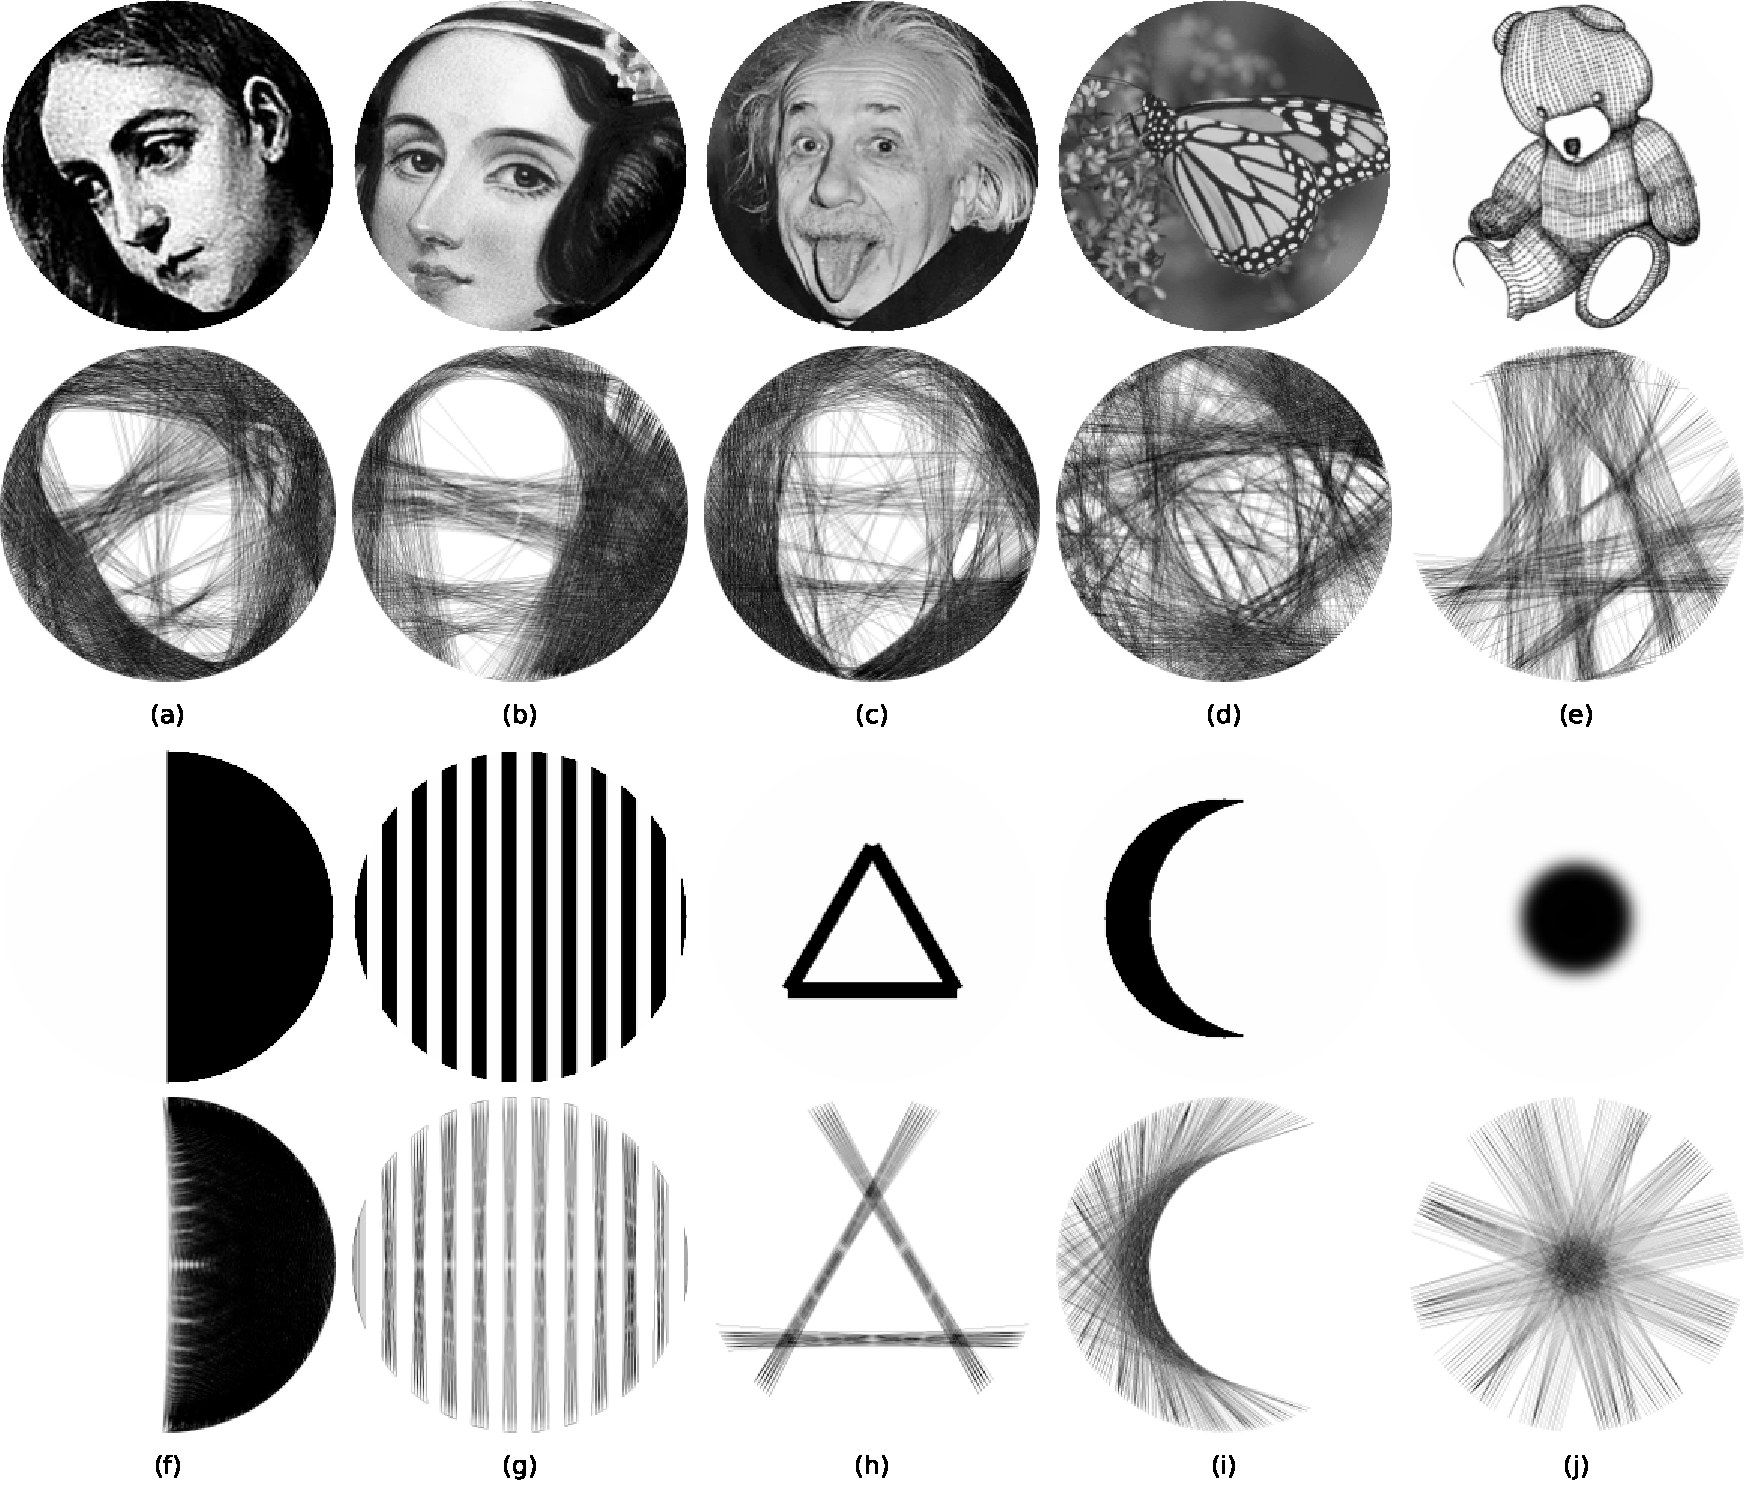
\includegraphics[width=\linewidth]{images/radon/radon_quantitative_test.pdf}
    \caption{Comparative analysis of reconstruction results using the Radon solver. The top image shows the input target image, while the bottom image displays the corresponding reconstruction. The solver was configured with 256 pegs and a patience factor of 10.}
    \label{fig:radon_quantitative}
\end{figure}

\begin{figure}[H]
    \centering
    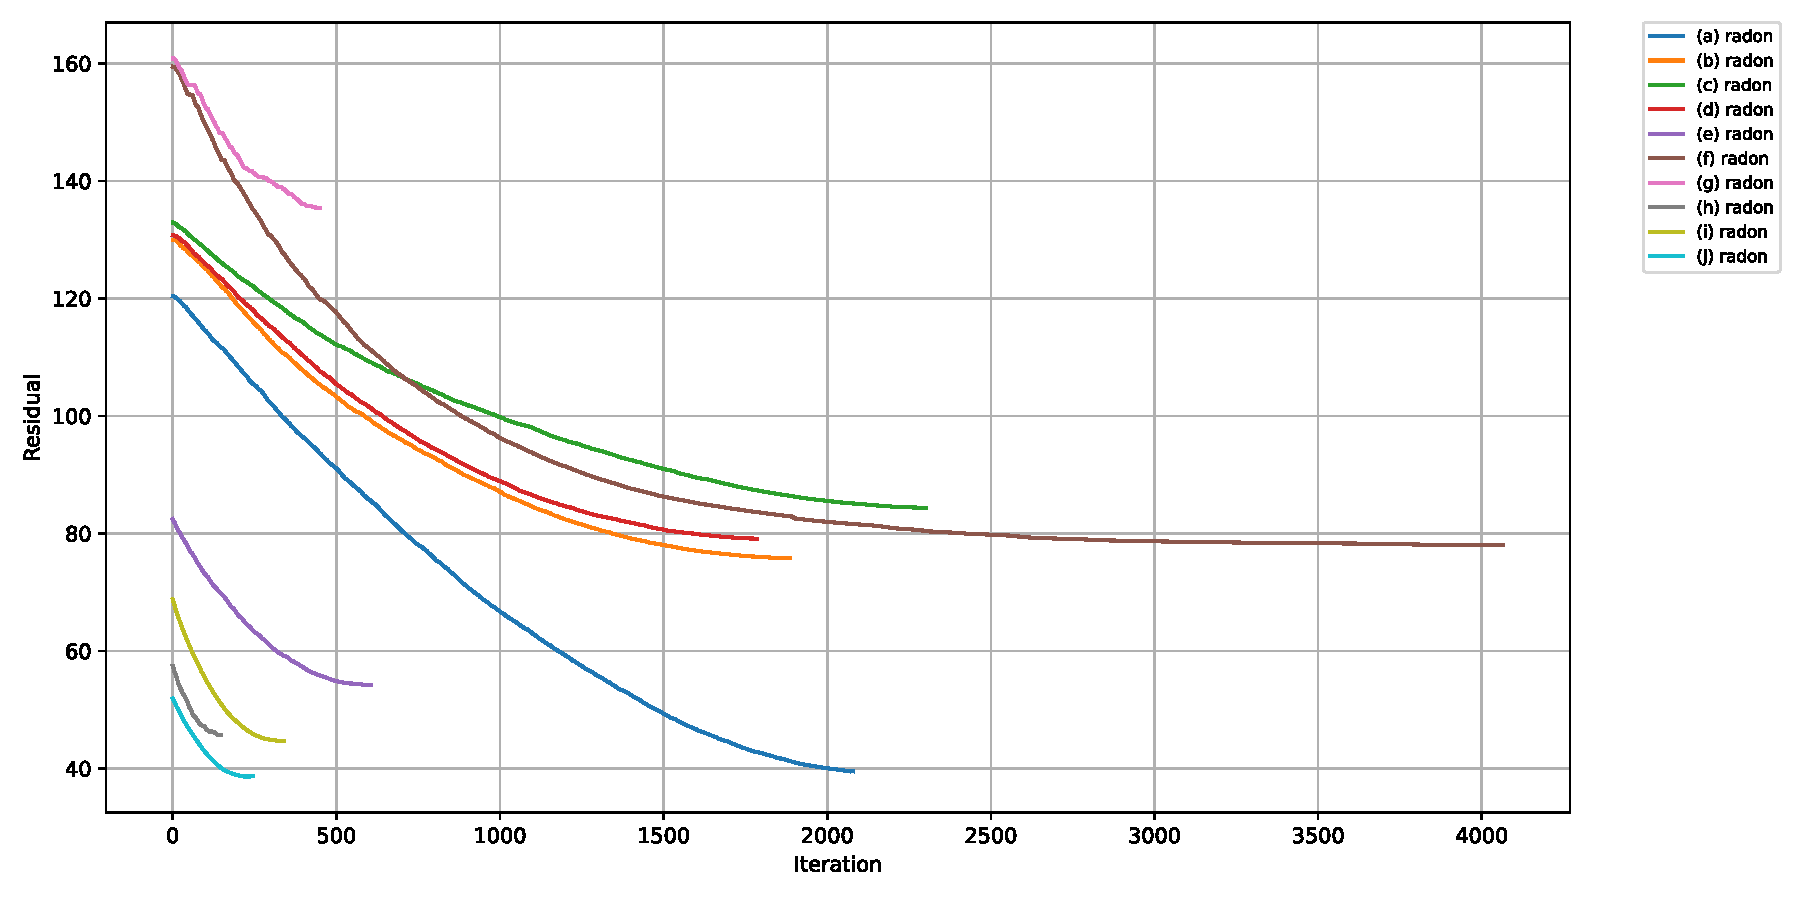
\includegraphics[width=\linewidth]{images/radon/residual_history.pdf}
    \caption{Residual error over iterations for each Radon solver.}
    \label{fig:radon_norm_error}
\end{figure}

\begin{table}[!ht]
\centering
\caption{Computation Time, Peak Memory Usage, RMS and number of Selected Lines for each Radon solver.}
\begin{tabularx}{\textwidth}{l C C C C}
\toprule
\textbf{Label} & \textbf{Computation Time (s)} & \textbf{Peak Memory Usage (MB)} & \textbf{RMS} & \textbf{Selected Lines} \\
\midrule
(a) & 2430            & 868.132            & 0.2557            & 1795 \\
(b) & 2406            & 868.131            & 0.1912            & 1579 \\
(c) & 2741            & 868.131            & 0.1906            & 1822 \\
(d) & 2159            & 868.131            & 0.2232            & 1538 \\
(e) &  821            & 868.131            & 0.2505            &  539 \\
(f) & 1216            & 868.132            & \textbf{0.1283}   & \textbf{2449} \\
(g) &  639            & 868.131            & 0.5104            &  312 \\
(h) &  \textbf{272}   & 868.131            & 0.2234            &   86 \\
(i) &  471            & 868.131            & 0.2266            &  323 \\
(j) &  375            & 868.131            & 0.2795            &  242 \\
\bottomrule
\end{tabularx}
\end{table}

\end{document}